% ============================================================
%  Informe – Proyecto Final de Cátedra 2026
%  Realidad Virtual – UNCuyo Ing.
% ============================================================
\documentclass[12pt, a4paper]{article}

% --- Encoding & Language ---
\usepackage[utf8]{inputenc}
\usepackage[T1]{fontenc}
\usepackage[spanish, es-tabla]{babel}

% --- Page Layout ---
\usepackage{geometry}
\geometry{
    a4paper,
    top=3.2cm,
    bottom=2.8cm,
    left=2.5cm,
    right=2.5cm,
    headheight=1.6cm,
    headsep=0.6cm,
    footskip=1.2cm
}

% --- Graphics & Color ---
\usepackage{graphicx}
\usepackage{pdflscape}
\usepackage[dvipsnames, table]{xcolor}

% --- Header / Footer ---
\usepackage{fancyhdr}
\usepackage{lastpage}

% --- Math & Other Utilities ---
\usepackage{amsmath, amssymb}
\usepackage{float}
\usepackage{url}
\usepackage{booktabs}
\usepackage{caption}

% --- Código fuente (estilo Go) ---
\usepackage{listings}

% Etiquetas en español y bloques indivisibles dentro de una página.
\renewcommand{\lstlistingname}{Código}
\renewcommand{\lstlistlistingname}{Índice de códigos}

\definecolor{gogreen}{rgb}{0.0, 0.50, 0.0}
\definecolor{goblue}{rgb}{0.0, 0.0, 0.75}
\definecolor{gogray}{rgb}{0.5, 0.5, 0.5}
\definecolor{gobg}{rgb}{0.97, 0.97, 0.97}

\lstdefinestyle{python}{
    float=htbp,
    language=Python,
    backgroundcolor=\color{gobg},
    basicstyle=\ttfamily\scriptsize,
    keywordstyle=\color{goblue}\bfseries,
    commentstyle=\color{gogreen}\itshape,
    stringstyle=\color{red},
    numberstyle=\tiny\color{gogray},
    numbers=left,
    numbersep=6pt,
    frame=single,
    framerule=0.4pt,
    rulecolor=\color{gogray},
    breaklines=true,
    breakatwhitespace=false,
    tabsize=4,
    showstringspaces=false,
    captionpos=b,
}

\lstdefinestyle{golang}{
    float=htbp,
    language=Go,
    backgroundcolor=\color{gobg},
    basicstyle=\ttfamily\footnotesize,
    keywordstyle=\color{goblue}\bfseries,
    commentstyle=\color{gogreen}\itshape,
    stringstyle=\color{red},
    numberstyle=\tiny\color{gogray},
    numbers=left,
    numbersep=6pt,
    frame=single,
    framerule=0.4pt,
    rulecolor=\color{gogray},
    breaklines=true,
    breakatwhitespace=false,
    tabsize=4,
    showstringspaces=false,
    captionpos=b,
}

\lstdefinestyle{csharp}{
    float=htbp,
    language=[Sharp]C,
    backgroundcolor=\color{gobg},
    basicstyle=\ttfamily\scriptsize,
    keywordstyle=\color{goblue}\bfseries,
    commentstyle=\color{gogreen}\itshape,
    stringstyle=\color{red},
    numberstyle=\tiny\color{gogray},
    numbers=left,
    numbersep=6pt,
    frame=single,
    framerule=0.4pt,
    rulecolor=\color{gogray},
    breaklines=true,
    breakatwhitespace=false,
    tabsize=4,
    showstringspaces=false,
    captionpos=b,
}

% \img: incluye imagen (el archivo debe existir)
\newcommand{\img}[2][width=\textwidth]{%
    \includegraphics[#1]{#2}%
}

% \imgpending: placeholder para imágenes aún no disponibles
\newcommand{\imgpending}[1]{%
    \begin{center}
        \fbox{\begin{minipage}{0.92\linewidth}
            \vspace{1.2cm}
            \centering\itshape\small
            [Imagen pendiente: \texttt{#1}]
            \vspace{1.2cm}
        \end{minipage}}
    \end{center}%
}

\usepackage{hyperref}
\hypersetup{hidelinks}

% ============================================================
%  COLORES
% ============================================================
\definecolor{azulUNC}{RGB}{0, 70, 127}
\definecolor{verdeRV}{RGB}{0, 110, 100}
\definecolor{grisLinea}{RGB}{90, 90, 90}

% ============================================================
%  ENCABEZADO Y PIE  (páginas del cuerpo)
% ============================================================
\pagestyle{fancy}
\fancyhf{}

\fancyhead[L]{%
    \footnotesize
    UNCuyo -- Facultad de Ingeniería \\
    Mendoza -- Argentina
}

\fancyhead[C]{%
    \footnotesize\bfseries
    Realidad Virtual (00318) \\
    PROYECTO FINAL DE CÁTEDRA
}

\fancyhead[R]{%
    \footnotesize
    Escobar, M. -- Martín Duci, I. \\
    Agosto 2026
}

\fancyfoot[C]{%
    \small\bfseries Pág.\ \thepage\ de \pageref{LastPage}
}

\renewcommand{\headrulewidth}{0.6pt}
\renewcommand{\footrulewidth}{0.6pt}

\renewcommand{\headrule}{%
    {\color{grisLinea}\hrule width\headwidth height\headrulewidth}%
    \vskip -\headrulewidth
}
\renewcommand{\footrule}{%
    {\color{grisLinea}\hrule width\headwidth height\footrulewidth}%
    \vskip -\footrulewidth
}

% ============================================================
%  DOCUMENTO
% ============================================================
\begin{document}

% ── PORTADA ─────────────────────────────────────────────────
\thispagestyle{empty}

\begin{center}

    \vspace*{1.5cm}

    {\large\bfseries
        Plataforma Interactiva de Realidad Virtual\\[5pt]
        para la Visualización de Soluciones de Ecuaciones Diferenciales Parciales\\[5pt]
        con Cómputo Remoto vía HTTP
    }

    \vspace{1.8cm}

    {\LARGE\bfseries\color{azulUNC} Universidad Nacional de Cuyo}\\[6pt]
    {\large Facultad de Ingeniería}

    \vspace{3cm}

    {\large\color{verdeRV}\bfseries Realidad Virtual (00318)}

    \vspace{0.4cm}

    {\normalsize Proyecto Final de Cátedra}

    \vspace{3cm}

    {\normalsize\bfseries Profesores}\\[6pt]
    {\normalsize\color{azulUNC}
        Prof. Rosenstein, Javier \\[4pt]
        Prof. Tomba, Carlos
    }

    \vspace{1.2cm}

    {\normalsize\bfseries Alumnos}\\[6pt]
    {\normalsize\color{azulUNC}
        Escobar, Matías \quad -- \quad 13328 \\[4pt]
        Martín Duci, Ignacio \quad -- \quad 13560
    }

    \vspace{1.2cm}

    {\normalsize Agosto 2026}
\end{center}

% ── ÍNDICE ──────────────────────────────────────────────────
\newpage
\thispagestyle{fancy}
\tableofcontents

% ── RESUMEN ─────────────────────────────────────────────────
\newpage
\thispagestyle{fancy}

\begin{center}
    {\large\bfseries Resumen}
\end{center}

\vspace{0.6cm}

El presente trabajo describe el desarrollo de un sistema cliente-servidor orientado al
entorno académico para el cálculo numérico y la visualización interactiva de ecuaciones
diferenciales parciales (EDPs). El sistema fue concebido como una plataforma de
exploración y aprendizaje que permite a los alumnos simular, probar e iterar sobre
distintas configuraciones de EDPs — variando parámetros físicos, condiciones iniciales
y dominios espaciales — para construir intuición sobre su comportamiento de forma
activa. Como funcionalidad complementaria, el sistema incorpora un mecanismo de
sincronización que permite al profesor propagar una configuración específica a todos
los dispositivos conectados, facilitando la discusión guiada en clase a partir de un
caso común.

El proyecto se estructura en dos componentes diferenciados. El primero corresponde al
\textbf{servidor}, implementado en el lenguaje \textbf{Go} utilizando el framework
\textbf{Gin} para la gestión de rutas HTTP. El servidor expone una API REST que permite
el registro de usuarios, el cálculo de soluciones numéricas y el control de
sincronización entre dispositivos. Se implementaron dos solvers de ecuaciones
diferenciales parciales: la \textbf{ecuación de onda 2D}, resuelta mediante el esquema
explícito \textit{leapfrog} de segundo orden con condición CFL, y la
\textbf{ecuación de calor 2D} sobre una placa cuadrada, resuelta mediante el esquema
\textit{FTCS} (\textit{Forward Time Centered Space}) explícito. Ambos solvers operan
sobre un dominio espacial discretizado con condiciones de contorno de Dirichlet, y
emplean técnicas de \textit{rolling buffer} y submuestreo temporal para mantener el
uso de memoria acotado independientemente de la duración de la simulación. El servidor
incluye además un panel web docente desarrollado en HTML, CSS y JavaScript, que permite
visualizar las soluciones en una representación tridimensional renderizada por software
mediante un rasterizador de polígonos implementado sobre el elemento \texttt{Canvas} de
HTML5, con controles de órbita y un sistema de sincronización de parámetros hacia los
alumnos.

El segundo componente corresponde a la \textbf{aplicación móvil}, desarrollada en
\textbf{Unity} y compilada para Android. La aplicación descubre automáticamente el
servidor dentro de la red local, registra al estudiante y consume las soluciones
numéricas completas sin ejecutar el método de diferencias finitas en el teléfono.
Los resultados se presentan sobre placas tridimensionales mediante color,
desplazamiento, grilla y nodos visibles. La cámara utiliza los sensores de orientación
del dispositivo y ofrece tanto una experiencia monoscópica a pantalla completa como un
modo estereoscópico opcional para Google Cardboard. El teléfono fue seleccionado como
dispositivo IHM porque constituye un recurso disponible para la totalidad de los alumnos
de la cátedra; por este motivo, el visor no es necesario para desarrollar la actividad.
El alumno puede modificar parámetros,
alternar entre onda y calor, desplazar la placa, explorar modos naturales y editar una
condición inicial seleccionando nodos. El cliente incorpora además una interfaz de
inicio adaptable a distintas pantallas Android y un coordinador que aplica las
configuraciones sincronizadas por el docente.

\vspace{0.4cm}
\noindent\textbf{Palabras clave:} ecuaciones diferenciales parciales, diferencias
finitas, Unity, Android, realidad virtual, Google Cardboard, arquitectura
cliente--servidor.

\vfill

% ── SECCIÓN 1: INTRODUCCIÓN ─────────────────────────────────
\newpage

\section{Introducción}

Las ecuaciones diferenciales parciales (EDPs) constituyen una de las herramientas
matemáticas fundamentales en ingeniería y ciencias aplicadas. Modelan fenómenos
físicos tan diversos como la propagación de ondas, la difusión de calor, el flujo de
fluidos y la deformación de estructuras. Sin embargo, su comprensión intuitiva
representa un desafío significativo para los estudiantes, en parte debido a que los
métodos de resolución analítica se limitan a casos muy particulares y las soluciones
numéricas suelen presentarse de forma estática en hojas de cálculo o gráficas
bidimensionales. Los métodos de diferencias finitas permiten aproximar estas soluciones
mediante una discretización espacial y temporal del problema continuo
\cite{leveque2007}.

El presente proyecto propone un enfoque alternativo: una plataforma interactiva que
permite al usuario simular el comportamiento de EDPs durante la ejecución, variar
libremente sus parámetros y condiciones iniciales, y observar las soluciones mediante
una visualización tridimensional controlada por la orientación del teléfono. El modo
plano concentra la interacción táctil, mientras que el modo Google Cardboard ofrece
renderizado estereoscópico y seguimiento rotacional de tres grados de libertad. El objetivo no es
reemplazar la teoría sino complementarla, ofreciendo un entorno donde la experimentación
directa genere intuición física sobre fenómenos que de otro modo resultan abstractos.

El sistema se compone de dos componentes principales que se comunican mediante una
arquitectura cliente-servidor HTTP. El servidor, desarrollado en Go, se encarga del
cálculo numérico de las soluciones y de gestionar múltiples clientes simultáneos. El
cliente, una aplicación móvil desarrollada en Unity, consume las soluciones del servidor
y las presenta en dos modalidades: una vista monoscópica interactiva y una vista
estereoscópica opcional orientada a Google Cardboard.

Como funcionalidad adicional orientada al uso en aula, el sistema incorpora un
mecanismo de sincronización que permite al profesor propagar una configuración
específica a todos los dispositivos conectados, habilitando la discusión guiada sobre
un caso común.

% ── SECCIÓN 2: OBJETIVOS Y BENEFICIARIOS ────────────────────
\newpage

\section{Objetivos y Beneficiarios}

\subsection{Objetivo general}

Desarrollar una plataforma cliente-servidor para la simulación interactiva de
ecuaciones diferenciales parciales, con visualización tridimensional y un modo de
realidad virtual opcional, que
facilite el aprendizaje activo mediante la exploración paramétrica de soluciones
numéricas en tiempo real.

\subsection{Objetivos específicos}

\begin{itemize}
    \item Implementar solvers numéricos estables y eficientes para la ecuación de onda
    2D y la ecuación de calor 2D sobre dominios cuadrados.

    \item Diseñar una API HTTP que exponga los resultados de la simulación a clientes
    heterogéneos (app móvil, panel web) de forma eficiente y con control de acceso por
    roles.

    \item Desarrollar una aplicación móvil en Unity que presente las soluciones
    numéricas en una escena tridimensional, permita la interacción táctil en modo plano
    y ofrezca visualización estereoscópica opcional para Google Cardboard.

    \item Proveer un panel web docente que permita visualizar, controlar y sincronizar
    simulaciones hacia múltiples usuarios conectados.

    \item Garantizar la estabilidad numérica de los esquemas implementados mediante el
    cumplimiento de las condiciones de estabilidad correspondientes a cada método.
\end{itemize}

\subsection{Beneficiarios}

La plataforma está orientada principalmente a \textbf{estudiantes de carreras de
ingeniería y ciencias exactas} que cursen asignaturas donde las EDPs tienen un rol
central: mecánica de medios continuos, transferencia de calor, electromagnetismo,
mecánica de fluidos, entre otras. La posibilidad de explorar libremente parámetros y
condiciones iniciales convierte al sistema en una herramienta de estudio autónomo que
complementa la clase magistral.

En segundo lugar, la plataforma beneficia a los \textbf{docentes}, que pueden utilizarla
como recurso didáctico durante la clase para ilustrar conceptos con simulaciones en
vivo, o proponer a los alumnos escenarios específicos mediante la funcionalidad de
sincronización.

% ── SECCIÓN 3: RESOLUCIÓN DE EDPs ───────────────────────────
\newpage

\section{Resolución de Ecuaciones Diferenciales}

\subsection{Fundamentos del método de diferencias finitas}

Las EDPs implementadas en este proyecto se resuelven mediante el \textbf{método de
diferencias finitas} (MDF), que consiste en discretizar el dominio continuo en una
grilla de puntos y aproximar las derivadas parciales mediante cocientes de diferencias
entre valores en nodos vecinos.

Dado un dominio espacial cuadrado $[0,L]\times[0,L]$ con $n$ subdivisiones, el paso
espacial es $\Delta x = \Delta y = L/n$. Los nodos interiores son los puntos
$(i\Delta x,\, j\Delta y)$ con $1 \leq i,j \leq n-2$. Las condiciones de contorno de
Dirichlet se imponen directamente sobre los nodos del borde, fijando su valor para
todo tiempo.

La aproximación por diferencias centradas de segundo orden para cada derivada segunda
espacial es:

\begin{equation}
    \frac{\partial^2 u}{\partial x^2} \approx
    \frac{u_{i+1,j} - 2\,u_{i,j} + u_{i-1,j}}{\Delta x^2}, \qquad
    \frac{\partial^2 u}{\partial y^2} \approx
    \frac{u_{i,j+1} - 2\,u_{i,j} + u_{i,j-1}}{\Delta y^2}
\end{equation}

El laplaciano $\nabla^2 u = \partial^2 u/\partial x^2 + \partial^2 u/\partial y^2$
se obtiene sumando ambas expresiones. Como el dominio es una grilla cuadrada uniforme
($\Delta x = \Delta y = L/n$), los dos denominadores son iguales y los términos en
$u_{i,j}$ se suman: $-2u_{i,j}/\Delta x^2 - 2u_{i,j}/\Delta y^2 = -4u_{i,j}/\Delta x^2$.
El resultado es el \textbf{laplaciano discreto de 5 puntos}:

\begin{equation}
    \nabla^2 u_{i,j} \approx
    \frac{u_{i+1,j} + u_{i-1,j} + u_{i,j+1} + u_{i,j-1} - 4\,u_{i,j}}{\Delta x^2}
    \label{eq:laplaciano}
\end{equation}

Esta expresión es la base de ambos esquemas numéricos implementados.

% ---- 3.1 -------------------------------------------------------
\subsection{Ecuación de onda 2D}

\subsubsection{Formulación matemática}

La ecuación de onda 2D base describe la evolución temporal de una membrana vibrante:

\begin{equation}
    \frac{\partial^2 u}{\partial t^2} = c^2
    \left(\frac{\partial^2 u}{\partial x^2} + \frac{\partial^2 u}{\partial y^2}\right)
    \label{eq:onda2d}
\end{equation}

La implementación extiende este modelo con amortiguamiento viscoso opcional y
excitación forzada armónica:

\begin{equation}
    \frac{\partial^2 u}{\partial t^2} + \gamma\frac{\partial u}{\partial t} =
    c^2\nabla^2 u + A\sin(2\pi f\,t)\,\phi(x,y)
    \label{eq:onda2d-ext}
\end{equation}

donde $u(x,y,t)$ es el desplazamiento de la membrana, $c$ la velocidad de propagación,
$\gamma \geq 0$ el coeficiente de amortiguamiento viscoso, $f$ la frecuencia de
excitación forzada [Hz] y $\phi(x,y)$ la forma espacial de la fuente. Se imponen
condiciones de contorno de Dirichlet homogéneas ($u = 0$ en todo el borde) y velocidad
inicial nula ($\partial u/\partial t\big|_{t=0} = 0$).

\subsubsection{Esquema leapfrog de segundo orden}

Se utiliza el esquema explícito \textit{leapfrog} centrado en tiempo y espacio, que
aproxima la derivada segunda temporal:

\begin{equation}
    \frac{\partial^2 u}{\partial t^2} \approx
    \frac{u^{k+1}_{i,j} - 2\,u^k_{i,j} + u^{k-1}_{i,j}}{\Delta t^2}
\end{equation}

El laplaciano del miembro derecho se aproxima aplicando la expresión~\eqref{eq:laplaciano}
definida en la sección anterior:

\begin{equation}
    c^2\!\left(\frac{\partial^2 u}{\partial x^2} + \frac{\partial^2 u}{\partial y^2}\right)
    = c^2\,\nabla^2 u \approx
    c^2\,\frac{u^k_{i+1,j} + u^k_{i-1,j} + u^k_{i,j+1} + u^k_{i,j-1} - 4\,u^k_{i,j}}
              {\Delta x^2}
\end{equation}

Sustituyendo esta expresión junto con la aproximación temporal en~\eqref{eq:onda2d}
se igualan ambos miembros:

\begin{equation}
    \frac{u^{k+1}_{i,j} - 2\,u^k_{i,j} + u^{k-1}_{i,j}}{\Delta t^2}
    = c^2\,
    \frac{u^k_{i+1,j} + u^k_{i-1,j} + u^k_{i,j+1} + u^k_{i,j-1} - 4\,u^k_{i,j}}
         {\Delta x^2}
\end{equation}

Multiplicando ambos miembros por $\Delta t^2$ y definiendo $r^2 = (c\,\Delta t/\Delta x)^2$:

\begin{equation}
    u^{k+1}_{i,j} - 2\,u^k_{i,j} + u^{k-1}_{i,j}
    = r^2\!\left(u^k_{i+1,j} + u^k_{i-1,j} + u^k_{i,j+1} + u^k_{i,j-1}
    - 4\,u^k_{i,j}\right)
\end{equation}

Despejando $u^{k+1}_{i,j}$:

\begin{equation}
    u^{k+1}_{i,j} = 2\,u^k_{i,j} - u^{k-1}_{i,j}
    + r^2\!\left(u^k_{i+1,j} + u^k_{i-1,j} + u^k_{i,j+1} + u^k_{i,j-1}
    - 4\,u^k_{i,j}\right)
    \label{eq:leapfrog}
\end{equation}

donde $r = c\,\Delta t / \Delta x$ es el \textbf{número de Courant}: mide cuántas
celdas espaciales recorre la perturbación en un paso temporal. Un valor $r > 1/\sqrt{2}$
significa que la perturbación ``salta'' más rápido de lo que el esquema puede
representar, provocando inestabilidad numérica.

Cuando se activa amortiguamiento ($\gamma > 0$) y/o excitación forzada, el esquema se
generaliza a:

\begin{equation}
\begin{split}
    u^{k+1}_{i,j} = \frac{1}{1+\gamma\Delta t}\Bigl[
    &\;2\,u^k_{i,j} - (1-\gamma\Delta t)\,u^{k-1}_{i,j} \\
    &+ r^2\!\left(u^k_{i+1,j}+u^k_{i-1,j}+u^k_{i,j+1}+u^k_{i,j-1}
       -4\,u^k_{i,j}\right) \\
    &+ A_{\rm exc}\sin(2\pi f\,t_k)\,\phi_{i,j}\Bigr]
\end{split}
    \label{eq:leapfrog-amort}
\end{equation}

donde $A_{\rm exc} = 0.15\,\Delta t^2$ escala la amplitud de la fuente y $\phi_{i,j}$
es su forma espacial, coincidente con el modo de vibración seleccionado:
\[
    \phi_{i,j} = \sin\!\left(\frac{m_1\pi x_i}{L}\right)\sin\!\left(\frac{m_2\pi y_j}{L}\right)
\]
Para $\gamma = 0$ y sin excitación el esquema se reduce a~\eqref{eq:leapfrog}.

Para el primer paso temporal, donde no existe $u^{k-1}$, se aplica la condición de
velocidad inicial nula para obtener un arranque de primer orden:

\begin{equation}
    u^1_{i,j} = u^0_{i,j} + \frac{r^2}{2}
    \left(u^0_{i+1,j} + u^0_{i-1,j} + u^0_{i,j+1} + u^0_{i,j-1}
    - 4\,u^0_{i,j}\right)
\end{equation}

\subsubsection{Condición de estabilidad CFL}

Para que el esquema leapfrog sea estable en 2D, el número de Courant debe satisfacer:

\begin{equation}
    r = \frac{c\,\Delta t}{\Delta x} \leq \frac{1}{\sqrt{2}}
    \label{eq:cfl-onda}
\end{equation}

En la implementación se usa $r = 0.9/\sqrt{2}$ para mantener un margen de seguridad.
El paso temporal resultante es $\Delta t = r\,\Delta x / c$, y el número de pasos
temporales necesario para simular $T$ segundos es $n_t = \lceil T / \Delta t \rceil$.

\subsubsection{Condiciones iniciales implementadas}

Se ofrecen tres configuraciones de condición inicial $u(x,y,0)$:

\begin{itemize}
    \item \textbf{Seno}: modo fundamental de vibración de la membrana cuadrada:
    \[u_0 = \sin\!\left(\frac{\pi x}{L}\right)\sin\!\left(\frac{\pi y}{L}\right)\]
    \item \textbf{Gaussiana}: pulso centrado que se propaga como ondas circulares:
    \[u_0 = \exp\!\left[-\left(\frac{x-L/2}{L/5}\right)^{\!2}
            -\left(\frac{y-L/2}{L/5}\right)^{\!2}\right]\]
    \item \textbf{Triangular}: pirámide lineal centrada:
    \[u_0 = \bigl(1-|2x/L-1|\bigr)\bigl(1-|2y/L-1|\bigr)\]
    \item \textbf{Modo $(m_1,m_2)$}: modo de vibración de orden superior, donde
    $m_1$ es la cantidad de semiondas a lo largo del eje $x$ y $m_2$ a lo largo del
    eje $y$, codificado como la cadena \texttt{"modo:$m_1$:$m_2$"} con
    $m_1,m_2\in\{1,\ldots,5\}$:
    \[u_0 = \sin\!\left(\frac{m_1\pi x}{L}\right)\sin\!\left(\frac{m_2\pi y}{L}\right)\]
    \item \textbf{Personalizada}: la app Unity puede enviar una grilla dibujada por el
    usuario (hasta $128\times128$ valores en el rango $[-2,2]$); el servidor la
    interpola bilinealmente a la resolución numérica interna antes de iniciar el solver.
\end{itemize}

% ---- 3.2 -------------------------------------------------------
\subsection{Ecuación de calor 2D}

\subsubsection{Formulación matemática}

La ecuación de calor 2D describe la difusión de temperatura sobre una placa cuadrada:

\begin{equation}
    \frac{\partial u}{\partial t} = \alpha
    \left(\frac{\partial^2 u}{\partial x^2} + \frac{\partial^2 u}{\partial y^2}\right)
    \label{eq:calor2d}
\end{equation}

donde $u(x,y,t)$ es la temperatura normalizada y $\alpha$ es la difusividad térmica del
material.

\subsubsection{Esquema FTCS explícito}

Se utiliza el esquema \textit{Forward Time Centered Space} (FTCS), que aproxima la
derivada temporal mediante diferencias hacia adelante de primer orden:

\begin{equation}
    \frac{\partial u}{\partial t} \approx
    \frac{u^{k+1}_{i,j} - u^k_{i,j}}{\Delta t}
\end{equation}

Sustituyendo ambas aproximaciones en la ecuación de calor~\eqref{eq:calor2d}:

\begin{equation}
    \frac{u^{k+1}_{i,j} - u^k_{i,j}}{\Delta t}
    = \alpha\,
    \frac{u^k_{i+1,j} + u^k_{i-1,j} + u^k_{i,j+1} + u^k_{i,j-1} - 4\,u^k_{i,j}}
         {\Delta x^2}
\end{equation}

Multiplicando ambos miembros por $\Delta t$ y definiendo $r_\alpha = \alpha\,\Delta t/\Delta x^2$,
y despejando $u^{k+1}_{i,j}$:

\begin{equation}
    u^{k+1}_{i,j} = u^k_{i,j} + r_\alpha\!
    \left(u^k_{i+1,j} + u^k_{i-1,j} + u^k_{i,j+1} + u^k_{i,j-1}
    - 4\,u^k_{i,j}\right)
    \label{eq:ftcs}
\end{equation}

donde $r_\alpha = \alpha\,\Delta t / \Delta x^2$ es el número de difusión.

A diferencia del esquema leapfrog, el FTCS solo requiere el instante anterior para
avanzar en tiempo, lo que simplifica la implementación al necesitar únicamente dos
grillas en lugar de tres.

\subsubsection{Condición de estabilidad}

Para que el esquema FTCS sea estable en 2D, el número de difusión debe satisfacer:

\begin{equation}
    r_\alpha = \frac{\alpha\,\Delta t}{\Delta x^2} \leq \frac{1}{4}
    \label{eq:estab-calor}
\end{equation}

En la implementación se usa $r_\alpha = 0.20$ como margen de seguridad respecto al
límite teórico de $0.25$.

\subsubsection{Condiciones iniciales y de contorno implementadas}

Se ofrecen tres configuraciones:

\begin{itemize}
    \item \textbf{Gaussiana}: pulso de temperatura centrado. Los cuatro bordes se fijan
    en $u = 0$ (sumideros fríos). El calor se disipa hacia los bordes y la temperatura
    interior decae hasta equilibrarse en cero.

    \item \textbf{Bordes calientes}: los cuatro bordes se fijan en $u = 1$ (fuentes de
    calor constantes) y el interior comienza en $u = 0$. El calor penetra desde las
    paredes hacia el centro hasta alcanzar el estado estacionario $u = 1$ en todo el
    dominio.

    \item \textbf{Placa caliente}: el interior comienza en $u = 1$ y los cuatro bordes
    se fijan en $u = 0$ (sumideros fríos). El calor fluye desde el interior hacia los
    bordes hasta alcanzar el estado estacionario $u = 0$ en todo el dominio.
\end{itemize}

En ambos casos las condiciones de contorno se reimponen explícitamente después de cada
paso temporal para mantener el valor fijo en el borde independientemente de la difusión
numérica.

% ── SECCIÓN 4: ARQUITECTURA DEL SERVIDOR ────────────────────
\newpage

\thispagestyle{fancy}

\section{Arquitectura General e Interconexión}

La Figura~\ref{fig:arquitectura-interconexion} resume la organización completa del
sistema, los algoritmos numéricos ejecutados en Go y los flujos de información entre
el panel docente, el servidor y las aplicaciones Android. Las flechas continuas
distinguen el sentido de cada petición y respuesta; la flecha discontinua representa
la propagación de la configuración sincronizada por el docente.

\begin{figure}[H]
    \centering
    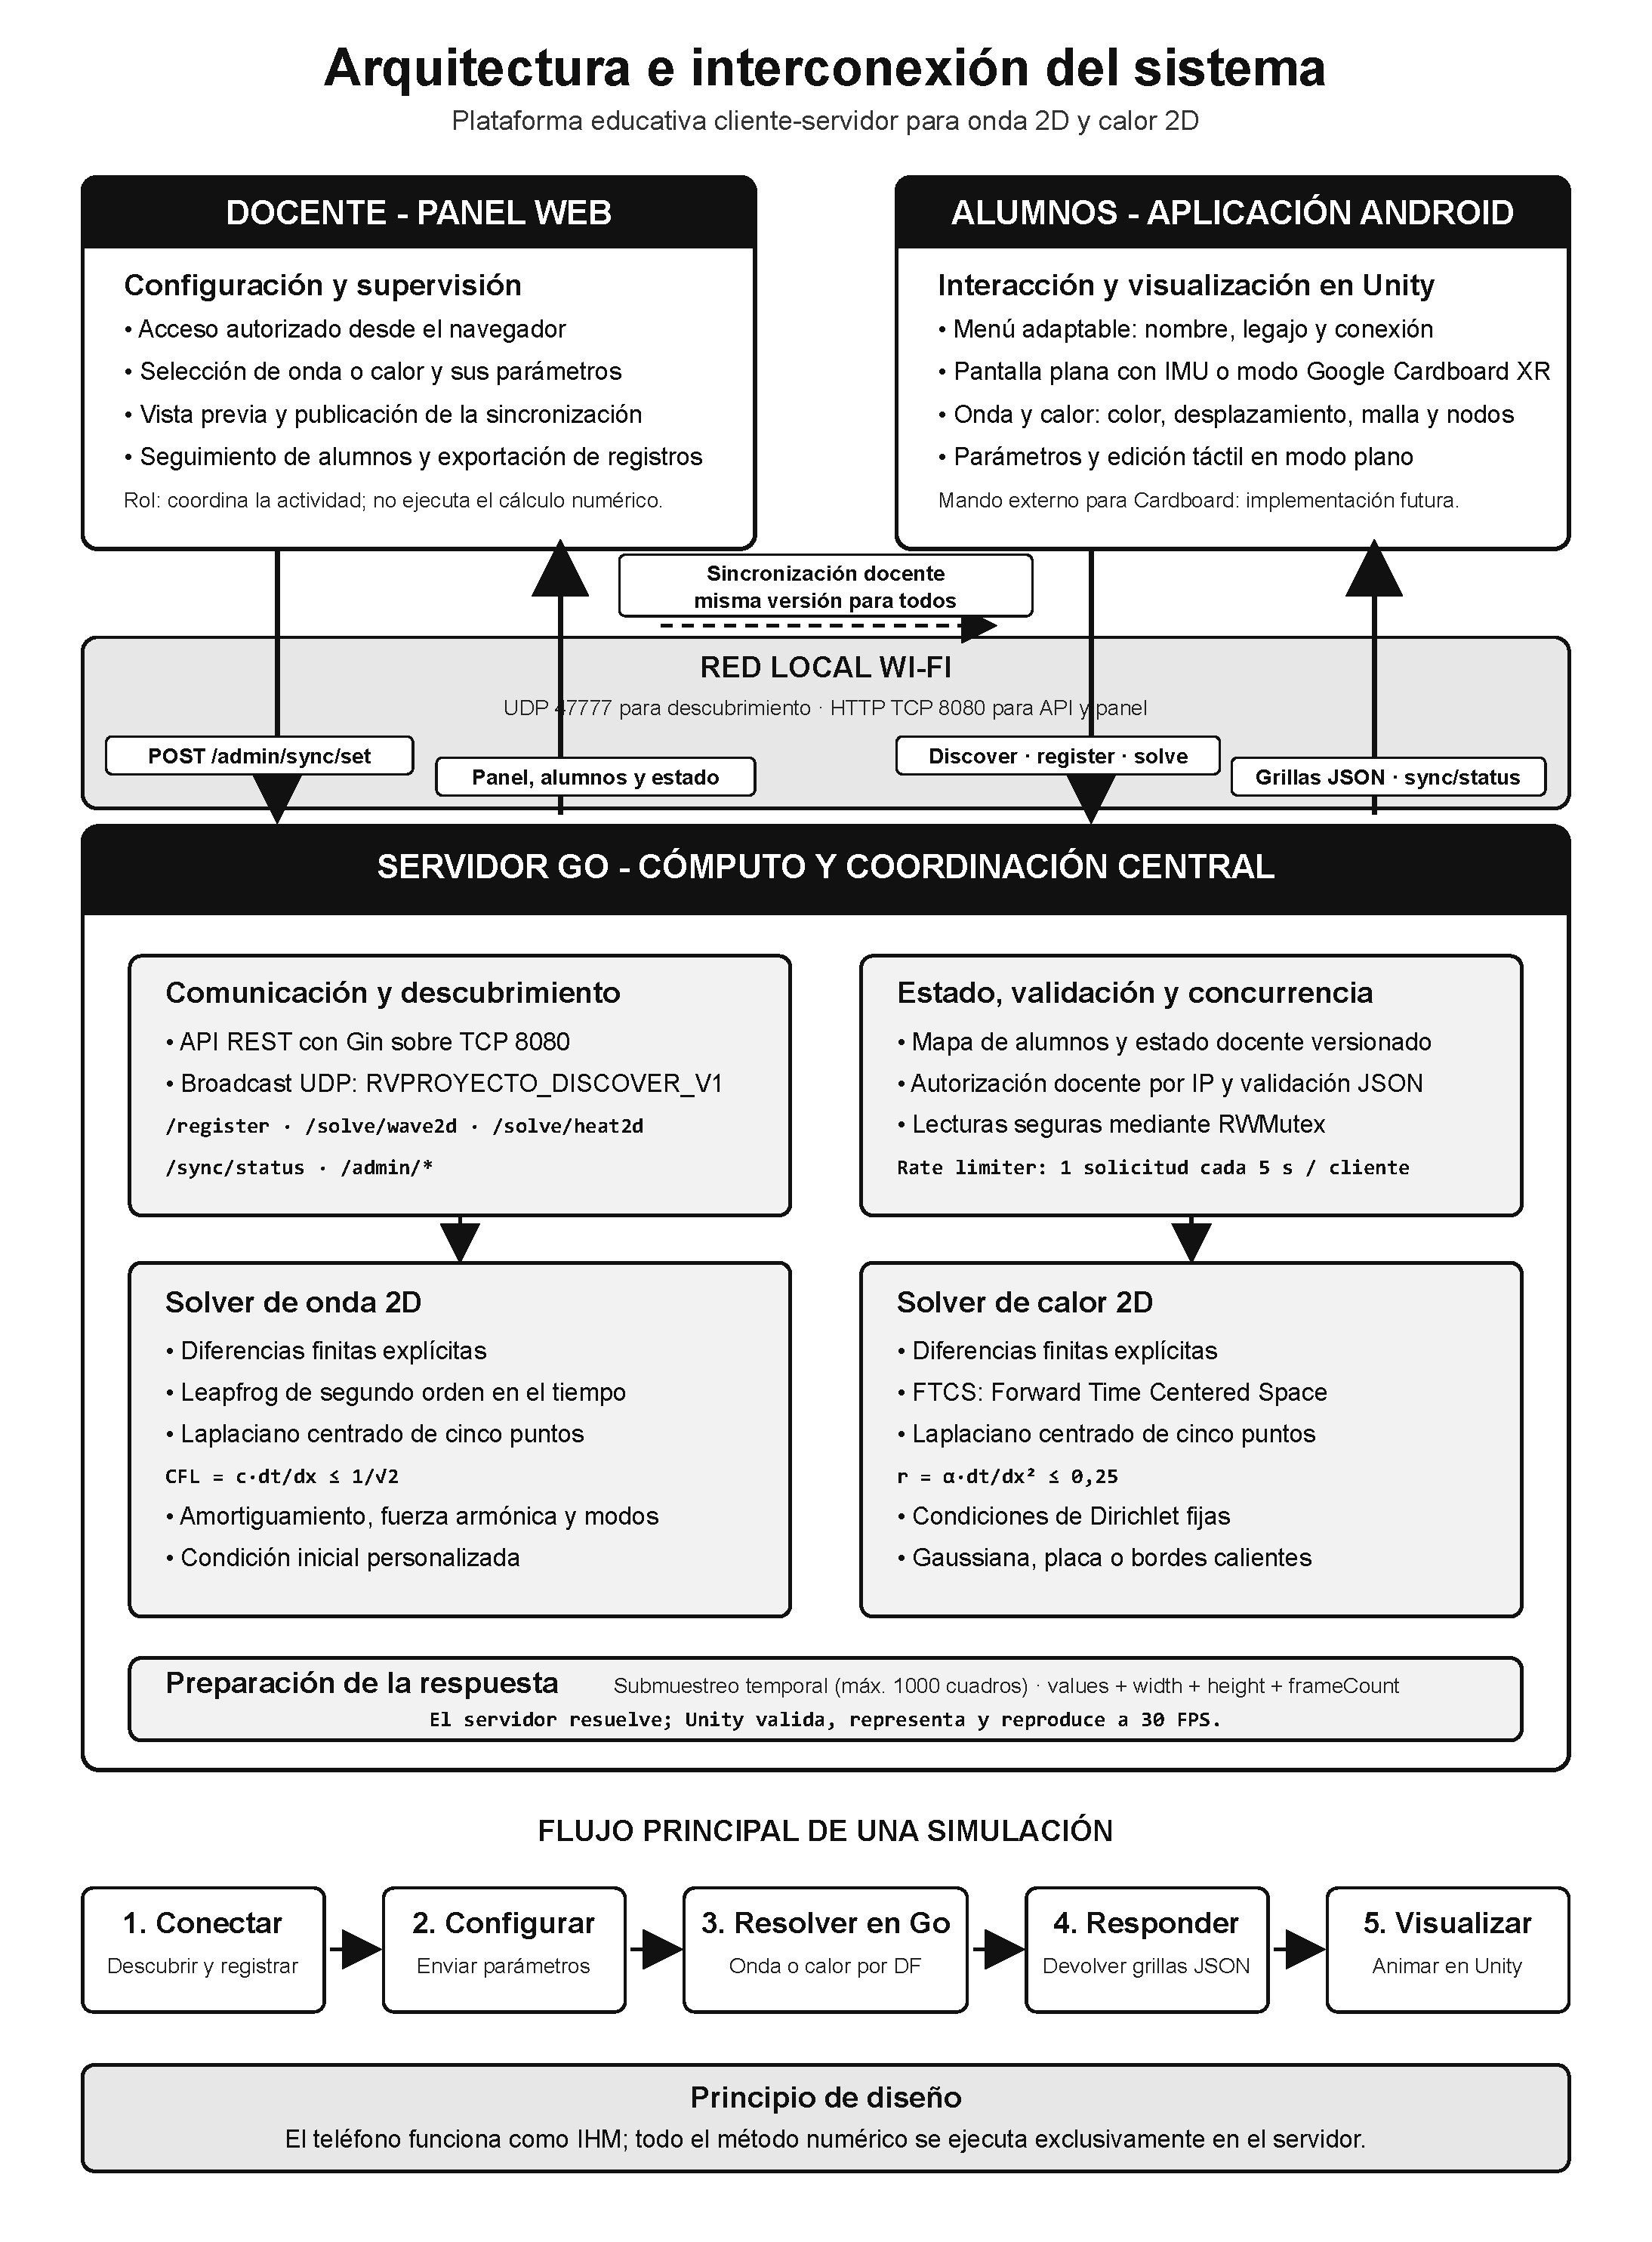
\includegraphics[width=0.98\linewidth,height=0.70\textheight,keepaspectratio]{diagramas/arquitectura_interconexion_bn.pdf}
    \caption{Arquitectura e interconexión de la plataforma. El servidor centraliza la
    comunicación, la sincronización y la resolución numérica; Unity representa las
    grillas recibidas y utiliza el teléfono como dispositivo IHM.}
    \label{fig:arquitectura-interconexion}
\end{figure}

\clearpage

\section{Arquitectura del Servidor}

El servidor está escrito íntegramente en Go y utiliza el marco de desarrollo
(\textit{framework}) \textbf{Gin} para la gestión de rutas HTTP
\cite{goDocs,ginDocs}. El código se organiza en nueve archivos, cada uno con una
responsabilidad bien delimitada:

\begin{center}
\begin{tabular}{ll}
\toprule
\textbf{Archivo} & \textbf{Responsabilidad} \\
\midrule
\texttt{main.go}      & Punto de entrada: flags CLI, GUI de lanzador y router \\
\texttt{gui.go}       & Lanzador gráfico en navegador; ciclo de vida del servidor \\
\texttt{auth.go}      & Autenticación del profesor y limitación de tasa por IP \\
\texttt{sync.go}      & Estado global en memoria: clientes, sincronización y versión \\
\texttt{handlers.go}  & Endpoints \texttt{/solve}, \texttt{/register} y \texttt{/sync/status} \\
\texttt{admin.go}     & Endpoints del panel web docente (\texttt{/admin/*}) \\
\texttt{wave\_api.go} & Endpoint \texttt{/solve/wave2d} dedicado a la app Unity (onda) \\
\texttt{heat\_api.go} & Endpoint \texttt{/solve/heat2d} dedicado a la app Unity (calor) \\
\texttt{solver.go}    & Solvers numéricos de EDPs (sin dependencias HTTP) \\
\bottomrule
\end{tabular}
\end{center}

Todos los archivos pertenecen al mismo paquete \texttt{main}, lo que significa que
comparten tipos, variables y funciones sin necesidad de importaciones entre ellos. El
estado global del servidor vive en una única variable (\texttt{estado}) definida en
\texttt{sync.go}, y todos los handlers acceden a ella mediante sus métodos.

\subsection{Resumen de rutas}

La tabla siguiente sintetiza todos los endpoints expuestos por el servidor, el método
HTTP, quién puede usarlos y qué devuelven.

\begin{center}
{\renewcommand{\arraystretch}{1.20}%
\setlength{\tabcolsep}{4pt}%
\footnotesize
\begin{tabular}{llll}
\toprule
\parbox[t]{3.5cm}{\textbf{Ruta}} & \parbox[t]{1.4cm}{\textbf{Método}} & \parbox[t]{2.5cm}{\textbf{Acceso}} & \parbox[t]{5.5cm}{\textbf{Función / Respuesta}} \\
\midrule
\parbox[t]{3.5cm}{\texttt{/}} & \parbox[t]{1.4cm}{GET} & \parbox[t]{2.5cm}{Todos} & \parbox[t]{5.5cm}{\raggedright Sirve el login del profesor (\texttt{login.html}).} \\
\parbox[t]{3.5cm}{\texttt{/auth}} & \parbox[t]{1.4cm}{POST} & \parbox[t]{2.5cm}{Todos} & \parbox[t]{5.5cm}{Verifica el código y autoriza su IP. Devuelve \texttt{\{ok:true\}}.} \\
\parbox[t]{3.5cm}{\texttt{/panel}} & \parbox[t]{1.4cm}{GET} & \parbox[t]{2.5cm}{Profesor} & \parbox[t]{5.5cm}{Sirve el panel docente; redirige al login si la IP no está autorizada.} \\
\parbox[t]{3.5cm}{\texttt{/register}} & \parbox[t]{1.4cm}{POST} & \parbox[t]{2.5cm}{App móvil} & \parbox[t]{5.5cm}{Registra o actualiza un alumno. Devuelve \texttt{\{ok:true\}}.} \\
\parbox[t]{3.5cm}{\texttt{/solve}} & \parbox[t]{1.4cm}{GET} & \parbox[t]{2.5cm}{Panel web} & \parbox[t]{5.5cm}{Calcula la EDP y devuelve \texttt{\{sync, ecuacion, result\}} con hasta 1000 frames.} \\
\parbox[t]{3.5cm}{\texttt{/solve/wave2d}} & \parbox[t]{1.4cm}{POST} & \parbox[t]{2.5cm}{App Unity} & \parbox[t]{5.5cm}{\raggedright Acepta parámetros de onda, amortiguamiento, excitación y condición personalizable; devuelve frames aplanados.} \\
\parbox[t]{3.5cm}{\texttt{/solve/heat2d}} & \parbox[t]{1.4cm}{POST} & \parbox[t]{2.5cm}{App Unity} & \parbox[t]{5.5cm}{Acepta parámetros térmicos y devuelve frames en el mismo formato aplanado.} \\
\parbox[t]{3.5cm}{\texttt{/sync/status}} & \parbox[t]{1.4cm}{GET} & \parbox[t]{2.5cm}{App móvil} & \parbox[t]{5.5cm}{Devuelve estado y versión de sincronización sin ejecutar el solver.} \\
\midrule
\parbox[t]{3.5cm}{\texttt{/admin/clients}} & \parbox[t]{1.4cm}{GET} & \parbox[t]{2.5cm}{Profesor} & \parbox[t]{5.5cm}{Lista alumnos con IP, legajo, nombre y último request.} \\
\parbox[t]{3.5cm}{\texttt{/admin/sync/set}} & \parbox[t]{1.4cm}{POST} & \parbox[t]{2.5cm}{Profesor} & \parbox[t]{5.5cm}{\raggedright Activa la sincronización, incluido amortiguamiento y excitación.} \\
\parbox[t]{3.5cm}{\texttt{/admin/sync/clear}} & \parbox[t]{1.4cm}{POST} & \parbox[t]{2.5cm}{Profesor} & \parbox[t]{5.5cm}{Desactiva la sincronización.} \\
\bottomrule
\end{tabular}}
\end{center}

% -------- main.go -----------------------------------------------
\subsection{\texttt{main.go} — Punto de entrada y router}

\texttt{main.go} declara la constante del código de acceso del profesor, interpreta
el flag de línea de comandos y decide entre arrancar la GUI de lanzador o el servidor
directamente. Las rutas se registran en \texttt{setupRouter()}, separando la
configuración del router de su ciclo de vida.

\begin{lstlisting}[style=golang, caption={\texttt{main.go} completo}]
package main

import (
    "flag"
    "github.com/gin-gonic/gin"
)

const codigoProfesor = "123"

func main() {
    port := flag.String("port", "", "puerto del servidor (omitir para usar la GUI)")
    flag.Parse()

    if *port != "" {
        startGinServer(*port)
    } else {
        runLauncherGUI()
    }
}

func setupRouter() *gin.Engine {
    router := gin.Default()

    router.StaticFile("/", "./web/login.html")
    router.StaticFile("/favicon.ico",  "./web/favicon.ico")
    // ... otros archivos estaticos de la webapp ...
    router.POST("/auth",  authHandler)
    router.GET("/panel",  panelHandler)

    admin := router.Group("/admin")
    {
        admin.GET("/clients",     clientesHandler)
        admin.POST("/sync/clear", syncClearHandler)
        admin.POST("/sync/set",   syncSetAdminHandler)
    }

    router.POST("/register",    registerHandler)
    router.GET("/sync/status",  syncStatusHandler)
    router.POST("/solve/wave2d", RateLimitMiddleware(), waveSolveUnityHandler)
    router.POST("/solve/heat2d", RateLimitMiddleware(), heatSolveUnityHandler)
    router.GET("/solve",         RateLimitMiddleware(), solveHandler)

    return router
}
\end{lstlisting}

Sin el flag \texttt{-port}, \texttt{main} llama a \texttt{runLauncherGUI()} (definida
en \texttt{gui.go}), que levanta un servidor HTTP local en un puerto efímero, abre el
navegador en esa dirección y queda a la espera: el usuario elige el puerto de red y
presiona ``Lanzar''. Con el flag, el servidor arranca directamente sin GUI, lo que
facilita el uso en scripts o despliegues automatizados.

\texttt{setupRouter()} centraliza el registro de todas las rutas. Existen tres
endpoints de cálculo: \texttt{/solve} para el panel web (array 3D), y
\texttt{/solve/wave2d} y \texttt{/solve/heat2d} para Unity (arrays 1D aplanados,
compatibles con \texttt{JsonUtility}). Los tres pasan por el rate limiter.
El nuevo endpoint \texttt{/sync/status} permite a la app consultar el estado de
sincronización sin ejecutar el solver, reduciendo el costo de las consultas de
\textit{polling}.

% -------- auth.go -----------------------------------------------
\subsection{\texttt{auth.go} — Autenticación y limitación de tasa}

Este archivo implementa dos mecanismos de control de acceso independientes: la
autenticación del profesor por IP y el limitador de tasa para los endpoints de cálculo.

\begin{lstlisting}[style=golang, caption={\texttt{auth.go} — imports y variables globales}]
package main

import (
    "fmt"
    "math"
    "net/http"
    "sync"
    "time"

    "github.com/gin-gonic/gin"
    "golang.org/x/time/rate"
)

type authRequest struct {
    Codigo string `json:"codigo"`
}

var (
    ipsAutorizadas   = make(map[string]bool)
    ipsAutorizadasMu sync.RWMutex
)

var limiters sync.Map
\end{lstlisting}

\texttt{ipsAutorizadas} actúa como lista blanca de IPs del profesor, protegido por su
propio \texttt{sync.RWMutex}. \texttt{limiters} es un \texttt{sync.Map} — mapa
concurrente sin mutex manual — que almacena un limitador de tasa por IP.

\begin{lstlisting}[style=golang, caption={Limitador de tasa por IP}]
func getLimiter(ip string) *rate.Limiter {
    if v, ok := limiters.Load(ip); ok {
        return v.(*rate.Limiter)
    }
    lim := rate.NewLimiter(rate.Every(5*time.Second), 1)
    actual, _ := limiters.LoadOrStore(ip, lim)
    return actual.(*rate.Limiter)
}

func RateLimitMiddleware() gin.HandlerFunc {
    return func(c *gin.Context) {
        ip := c.GetHeader("X-Forwarded-For")
        if ip == "" {
            ip = c.ClientIP()
        }
        lim := getLimiter(ip)

        res := lim.Reserve()
        if !res.OK() {
            c.AbortWithStatusJSON(http.StatusTooManyRequests,
                gin.H{"error": "Demasiadas peticiones"})
            return
        }

        delay := res.Delay()
        if delay <= 0 {
            c.Next()
            return
        }

        res.Cancel()
        sec := int(math.Ceil(delay.Seconds()))
        c.Header("Retry-After", fmt.Sprintf("%d", sec))
        c.AbortWithStatusJSON(http.StatusTooManyRequests, gin.H{
            "error":       "Demasiadas peticiones",
            "waitSeconds": sec,
            "message":     fmt.Sprintf("Espera %ds antes de reintentar", sec),
        })
    }
}
\end{lstlisting}

El middleware lee primero la cabecera \texttt{X-For\-war\-ded-For} antes de caer en
\texttt{c.Client\-IP()}: esto permite identificar la IP real del cliente cuando
el servidor corre detrás de un proxy o balanceador de carga. El limitador usa el
patrón \textit{token bucket}: un token se regenera cada cinco segundos. Si el token
no está disponible, se calcula el tiempo de espera, se cancela la reserva (para no
consumirlo) y se responde 429 con la cabecera \texttt{Retry-After}.

\begin{lstlisting}[style=golang, caption={Autenticación del profesor}]
func autorizarIP(ip string) {
    ipsAutorizadasMu.Lock()
    defer ipsAutorizadasMu.Unlock()
    ipsAutorizadas[ip] = true
    fmt.Println("[auth] IP autorizada:", ip)
}

func ipAutorizada(ip string) bool {
    ipsAutorizadasMu.RLock()
    defer ipsAutorizadasMu.RUnlock()
    return ipsAutorizadas[ip]
}

func authHandler(c *gin.Context) {
    var req authRequest
    if err := c.ShouldBindJSON(&req); err != nil {
        c.JSON(http.StatusBadRequest,
            gin.H{"error": "Cuerpo de solicitud invalido"})
        return
    }
    if req.Codigo != codigoProfesor {
        c.JSON(http.StatusUnauthorized, gin.H{"error": "Codigo incorrecto"})
        return
    }
    autorizarIP(c.ClientIP())
    c.JSON(http.StatusOK, gin.H{"ok": true})
}

func panelHandler(c *gin.Context) {
    if !ipAutorizada(c.ClientIP()) {
        c.Redirect(http.StatusFound, "/")
        return
    }
    c.File("./web/panel.html")
}
\end{lstlisting}

\texttt{panelHandler} redirige al login en lugar de devolver un error HTTP, para que
el flujo sea transparente en el navegador del profesor.

% -------- sync.go -----------------------------------------------
\subsection{\texttt{sync.go} — Estado global en memoria}

Este archivo centraliza todo el estado compartido entre handlers. El sistema de roles
de asistente fue eliminado: \texttt{Cliente} ya no tiene campo \texttt{Rol}, y
\texttt{parametrosSync} se extendió para incluir los parámetros de amortiguamiento
y excitación forzada.

\begin{lstlisting}[style=golang, caption={\texttt{sync.go} — tipos y estado global}]
package main

import (
    "sync"
    "time"
)

type Cliente struct {
    IP            string
    Legajo        string
    Nombre        string
    UltimoRequest time.Time
}

type parametrosSync struct {
    Ecuacion        string
    L               float64
    T               float64
    C               float64
    Inicial         string
    Amortiguamiento bool
    Gamma           float64
    Excitacion      bool
    FormaExcitacion string
    FrecExcitacion  float64
}

type estadoGlobal struct {
    mu       sync.RWMutex
    clientes map[string]*Cliente
    sync     struct {
        activo     bool
        parametros parametrosSync
        version    uint64  // incrementa en cada ActivarSync / DesactivarSync
    }
}

var estado = &estadoGlobal{
    clientes: make(map[string]*Cliente),
}
\end{lstlisting}

Los campos de \texttt{parametrosSync} permiten que el profesor sincronice no solo la
ecuación y sus parámetros básicos, sino también el amortiguamiento viscoso ($\gamma$) y
la excitación forzada (frecuencia y forma). El campo \texttt{version} es un contador
monótonamente creciente: se incrementa en cada \texttt{ActivarSync} y
\texttt{DesactivarSync}, lo que permite a los clientes detectar un cambio con una
consulta liviana a \texttt{/sync/status} sin tener que re-ejecutar el solver.

\begin{lstlisting}[style=golang, caption={Registro y consulta de clientes}]
func (e *estadoGlobal) RegistrarCliente(ip, legajo, nombre string) {
    e.mu.Lock()
    defer e.mu.Unlock()

    if c, existe := e.clientes[ip]; existe {
        c.Legajo = legajo
        c.Nombre = nombre
        c.UltimoRequest = time.Now()
        return
    }

    e.clientes[ip] = &Cliente{
        IP:            ip,
        Legajo:        legajo,
        Nombre:        nombre,
        UltimoRequest: time.Now(),
    }
}

func (e *estadoGlobal) ActualizarRequest(ip string) {
    e.mu.Lock()
    defer e.mu.Unlock()
    if c, existe := e.clientes[ip]; existe {
        c.UltimoRequest = time.Now()
    }
}

func (e *estadoGlobal) Clientes() []*Cliente {
    e.mu.RLock()
    defer e.mu.RUnlock()
    lista := make([]*Cliente, 0, len(e.clientes))
    for _, c := range e.clientes {
        lista = append(lista, c)
    }
    return lista
}
\end{lstlisting}

\texttt{RegistrarCliente} es idempotente: si la IP ya existe, actualiza legajo y nombre
preservando el resto del estado. Las operaciones de lectura usan \texttt{RLock}
(múltiples lectores simultáneos); las de escritura usan \texttt{Lock} (exclusividad).
\texttt{defer} garantiza la liberación del mutex incluso ante un panic.

\begin{lstlisting}[style=golang, caption={Control de sincronizacion}]
func (e *estadoGlobal) ActivarSync(p parametrosSync) {
    e.mu.Lock()
    defer e.mu.Unlock()
    e.sync.activo = true
    e.sync.parametros = p
    e.sync.version++
}

func (e *estadoGlobal) DesactivarSync() {
    e.mu.Lock()
    defer e.mu.Unlock()
    e.sync.activo = false
    e.sync.parametros = parametrosSync{}
    e.sync.version++
}

func (e *estadoGlobal) EstadoSync() (bool, parametrosSync) {
    e.mu.RLock()
    defer e.mu.RUnlock()
    return e.sync.activo, e.sync.parametros
}

// EstadoSyncVersionado permite detectar cambios sin re-ejecutar el solver.
func (e *estadoGlobal) EstadoSyncVersionado() (bool, parametrosSync, uint64) {
    e.mu.RLock()
    defer e.mu.RUnlock()
    return e.sync.activo, e.sync.parametros, e.sync.version
}
\end{lstlisting}

La sincronización funciona como difusión pasiva: el profesor escribe los parámetros
una vez, y cualquier cliente que llame a \texttt{/solve}, \texttt{/solve/wave2d} o
\texttt{/solve/heat2d} recibe esos parámetros en lugar de los propios. No hay
websockets ni notificaciones push. El campo \texttt{"sync": true} en la respuesta
indica al cliente que los parámetros fueron impuestos. La app puede además consultar
\texttt{GET /sync/status} para obtener el campo \texttt{"version"}: si el número
cambió respecto al último guardado, hay una nueva configuración que descargar.

% -------- handlers.go -------------------------------------------
\subsection{\texttt{handlers.go} — Endpoints del panel web}

Este archivo implementa el registro de alumnos, el endpoint \texttt{/solve} utilizado
por el panel web y el nuevo \texttt{/sync/status}. El solver de onda 2D acepta
parámetros adicionales de amortiguamiento y excitación forzada, y el panel puede
seleccionar modos de vibración superiores mediante los query params \texttt{modoA} y
\texttt{modoB} (codificados internamente como \texttt{"modo:$m_1$:$m_2$"}).

\begin{lstlisting}[style=golang, caption={\texttt{handlers.go} — registro de alumno}]
package main

import (
    "net/http"
    "strconv"
    "github.com/gin-gonic/gin"
)

type registerRequest struct {
    Legajo string `json:"legajo"`
    Nombre string `json:"nombre"`
}

func registerHandler(c *gin.Context) {
    var req registerRequest
    if err := c.ShouldBindJSON(&req); err != nil {
        c.JSON(http.StatusBadRequest,
            gin.H{"error": "Cuerpo de solicitud invalido"})
        return
    }
    if req.Legajo == "" || req.Nombre == "" {
        c.JSON(http.StatusBadRequest,
            gin.H{"error": "Legajo y nombre son obligatorios"})
        return
    }
    estado.RegistrarCliente(c.ClientIP(), req.Legajo, req.Nombre)
    c.JSON(http.StatusOK, gin.H{"ok": true})
}
\end{lstlisting}

\begin{lstlisting}[style=golang, caption={Inicio del cálculo y aplicación de la sincronización}]
func solveHandler(c *gin.Context) {
    estado.ActualizarRequest(c.ClientIP())
    syncActivo, params := estado.EstadoSync()

    var L, T, cw, gamma float64
    var inicial, ecuacion string
    var amortiguamiento bool
    var exc excitacionOpts

    if syncActivo {
        L               = params.L
        T               = params.T
        cw              = params.C
        inicial         = params.Inicial
        ecuacion        = params.Ecuacion
        amortiguamiento = params.Amortiguamiento
        gamma           = params.Gamma
        exc = excitacionOpts{
            Activa:     params.Excitacion,
            Forma:      params.FormaExcitacion,
            Frecuencia: params.FrecExcitacion,
        }
    }
    // Si no hay sincronizacion, se leen los datos del alumno.
}
\end{lstlisting}

\begin{lstlisting}[style=golang, caption={Lectura y validación de los parámetros de cálculo}]
if !syncActivo {
        // Continuacion de solveHandler.
        Ls, ok1 := c.GetQuery("L")
        Ts, ok2 := c.GetQuery("T")
        cs, ok3 := c.GetQuery("c")
        inicial, _  = c.GetQuery("inicial")
        ecuacion, _ = c.GetQuery("ecuacion")

        if !ok1 || !ok2 || !ok3 {
            c.JSON(http.StatusBadRequest,
                gin.H{"error": "Faltan parametros en la consulta"})
            return
        }

        var err1, err2, err3 error
        L,  err1 = strconv.ParseFloat(Ls, 64)
        T,  err2 = strconv.ParseFloat(Ts, 64)
        cw, err3 = strconv.ParseFloat(cs, 64)

        if err1 != nil || err2 != nil || err3 != nil {
            c.JSON(http.StatusBadRequest, gin.H{"error": "Parametros invalidos"})
            return
        }

        lMax := 10.0
        if ecuacion == "calor2d" { lMax = 20.0 }
        if L < 1 || L > lMax || T < 1 || T > 100 || cw < 0.1 || cw > 2 {
            c.JSON(http.StatusBadRequest,
                gin.H{"error": "Parametros fuera de rango"})
            return
        }

        if gs, ok := c.GetQuery("gamma"); ok {
            if g, err := strconv.ParseFloat(gs, 64); err == nil &&
                g >= 0 && g <= 1 {
                gamma = g
                amortiguamiento = gamma > 0
            }
        }

        if fs, ok := c.GetQuery("frecExcitacion"); ok {
            if f, err := strconv.ParseFloat(fs, 64); err == nil &&
                f > 0 && f <= 20 {
                forma, _ := c.GetQuery("formaExcitacion")
                if forma == "" { forma = "seno" }
                exc = excitacionOpts{Activa: true, Forma: forma, Frecuencia: f}
            }
        }
}
\end{lstlisting}

\begin{lstlisting}[style=golang, caption={Selección del solver y construcción de la respuesta}]
// Tramo final de solveHandler.
    var result interface{}
    switch ecuacion {
    case "calor2d":
        result = ecuacion_calor_2d(L, T, cw, inicial)
    default:
        ecuacion = "onda2d"
        effectiveGamma := 0.0
        if amortiguamiento { effectiveGamma = gamma }
        result = ecuacion_onda_2d(L, T, cw, effectiveGamma, exc, inicial)
    }

    c.JSON(http.StatusOK, gin.H{
        "sync":     syncActivo,
        "ecuacion": ecuacion,
        "result":   result,
    })
\end{lstlisting}

Los parámetros opcionales \texttt{gamma} (amortiguamiento) y
\texttt{frecExcitacion} (excitación forzada) se leen solo si están presentes en la
URL: si el valor de \texttt{gamma} es mayor que cero se activa el amortiguamiento; si
\texttt{frecExcitacion} es válido se construye el struct \texttt{excitacionOpts} con la
frecuencia y la forma de onda indicadas. Cuando \texttt{inicial=modo}, los query params
\texttt{modoA} y \texttt{modoB} especifican los índices del modo; ambos se validan en
el rango $[1,5]$ antes de codificarse como \texttt{"modo:$m_1$:$m_2$"}.

\texttt{syncStatusHandler} (en el mismo archivo, no listado aquí por brevedad) atiende
\texttt{GET /sync/status}: llama a \texttt{EstadoSyncVersionado()} y devuelve el estado
completo junto con el número de versión, sin ejecutar ningún solver.

% -------- wave_api.go -------------------------------------------
\subsection{\texttt{wave\_api.go} — Endpoint dedicado a Unity}

Este archivo implementa el endpoint \texttt{POST /solve/wave2d}, diseñado
específicamente para la aplicación Unity. La diferencia principal respecto a
\texttt{/solve} es el formato de respuesta: Unity usa \texttt{JsonUtility}, que no
puede deserializar arrays de arrays anidados, por lo que los frames se aplanan en un
único array 1D.

\begin{lstlisting}[style=golang, caption={\texttt{wave\_api.go} — estructuras de entrada y salida}]
package main

import (
    "math"
    "net/http"
    "github.com/gin-gonic/gin"
)

type waveSolveRequest struct {
    L               float64   `json:"l"`
    T               float64   `json:"t"`
    C               float64   `json:"c"`
    Inicial         string    `json:"inicial"`
    Amortiguamiento bool      `json:"amortiguamiento"`
    Gamma           float64   `json:"gamma"`
    Excitacion      bool      `json:"excitacion"`
    FormaExcitacion string    `json:"formaExcitacion"`
    FrecExcitacion  float64   `json:"frecExcitacion"`
    InitialWidth    int       `json:"initialWidth"`
    InitialHeight   int       `json:"initialHeight"`
    InitialValues   []float64 `json:"initialValues"`
}

type waveParametersResponse struct {
    L               float64 `json:"l"`
    T               float64 `json:"t"`
    C               float64 `json:"c"`
    Inicial         string  `json:"inicial"`
    Amortiguamiento bool    `json:"amortiguamiento"`
    Gamma           float64 `json:"gamma"`
}

type waveGridResponse struct {
    Width      int       `json:"width"`
    Height     int       `json:"height"`
    FrameCount int       `json:"frameCount"`
    Values     []float32 `json:"values"`
}

type waveSolveResponse struct {
    Sync       bool                   `json:"sync"`
    Ecuacion   string                 `json:"ecuacion"`
    Parametros waveParametersResponse `json:"parametros"`
    Result     waveGridResponse       `json:"result"`
}
\end{lstlisting}

\texttt{waveGridResponse} aplana los frames en un array \texttt{Values} de tipo
\texttt{[]float32} (precisión simple para reducir el tamaño de la respuesta JSON). El
valor en la posición $(frame, x, y)$ se obtiene con el índice\\
\texttt{frame*width*height + x*height + y}.
\texttt{waveParametersResponse} devuelve los parámetros efectivamente usados, que
pueden diferir de los solicitados si hay sincronización activa.

\begin{lstlisting}[style=golang, caption={\texttt{wave\_api.go} — handler principal}]
func waveSolveUnityHandler(c *gin.Context) {
    estado.ActualizarRequest(c.ClientIP())

    var req waveSolveRequest
    if err := c.ShouldBindJSON(&req); err != nil {
        c.JSON(http.StatusBadRequest, gin.H{"error": "Cuerpo de solicitud invalido"})
        return
    }

    syncActivo, syncParams := estado.EstadoSync()
    if syncActivo {
        req.L               = syncParams.L
        req.T               = syncParams.T
        req.C               = syncParams.C
        req.Inicial         = syncParams.Inicial
        req.Amortiguamiento = syncParams.Amortiguamiento
        req.Gamma           = syncParams.Gamma
        req.Excitacion      = syncParams.Excitacion
        req.FormaExcitacion = syncParams.FormaExcitacion
        req.FrecExcitacion  = syncParams.FrecExcitacion
        req.InitialWidth    = 0
        req.InitialHeight   = 0
        req.InitialValues   = nil
    }

    if req.L < 1 || req.L > 10 || req.T < 1 || req.T > 100 ||
        req.C < 0.1 || req.C > 2 {
        c.JSON(http.StatusBadRequest, gin.H{"error": "Parametros fuera de rango"})
        return
    }
\end{lstlisting}

La sincronización sobreescribe todos los parámetros del request, incluyendo los campos
de condición inicial personalizada (\texttt{InitialWidth}, \texttt{InitialHeight},
\texttt{InitialValues}), que se anulan porque la sincronización no admite grillas
dibujadas por el usuario.

\begin{lstlisting}[style=golang, caption={Validación de la condición inicial de la onda}]
    switch req.Inicial {
    case "seno", "triangular", "gauss":
        // valido
    case "personalizada":
        if req.InitialWidth < 2 || req.InitialWidth > 128 ||
            req.InitialHeight < 2 || req.InitialHeight > 128 ||
            len(req.InitialValues) != req.InitialWidth*req.InitialHeight {
            c.JSON(http.StatusBadRequest,
                gin.H{"error": "Grilla inicial personalizada invalida"})
            return
        }
        for _, value := range req.InitialValues {
            if math.IsNaN(value) || math.IsInf(value, 0) ||
                value < -2 || value > 2 {
                c.JSON(http.StatusBadRequest,
                    gin.H{"error": "Valores iniciales fuera de rango"})
                return
            }
        }
    default:
        c.JSON(http.StatusBadRequest,
            gin.H{"error": "Condicion inicial invalida"})
        return
    }
\end{lstlisting}

La condición inicial \texttt{"personalizada"} permite a Unity enviar una grilla
dibujada por el usuario (hasta 128x128). El servidor valida que las dimensiones y
valores sean correctos y que no haya NaN ni Inf antes de pasarlos al solver, ya que
estos valores romperían el esquema leapfrog.

\begin{lstlisting}[style=golang, caption={Cálculo y construcción de la respuesta de onda}]
    effectiveGamma := 0.0
    if req.Amortiguamiento && req.Gamma >= 0 && req.Gamma <= 1 {
        effectiveGamma = req.Gamma
    }

    exc := excitacionOpts{}
    if req.Excitacion && req.FrecExcitacion > 0 && req.FrecExcitacion <= 20 {
        forma := req.FormaExcitacion
        if forma == "" { forma = "seno" }
        exc = excitacionOpts{Activa: true, Forma: forma, Frecuencia: req.FrecExcitacion}
    }

    var frames [][][]float64
    if req.Inicial == "personalizada" {
        frames = ecuacion_onda_2d_personalizada(
            req.L, req.T, req.C, effectiveGamma, exc,
            req.InitialValues, req.InitialWidth, req.InitialHeight,
        )
    } else {
        frames = ecuacion_onda_2d(req.L, req.T, req.C, effectiveGamma, exc, req.Inicial)
    }
    result := flattenWaveFrames(frames)

    c.JSON(http.StatusOK, waveSolveResponse{
        Sync:     syncActivo,
        Ecuacion: "onda2d",
        Parametros: waveParametersResponse{
            L: req.L, T: req.T, C: req.C, Inicial: req.Inicial,
            Amortiguamiento: req.Amortiguamiento, Gamma: effectiveGamma,
        },
        Result: result,
    })
}
\end{lstlisting}

\begin{lstlisting}[style=golang, caption={Aplanamiento de frames para Unity}]
func flattenWaveFrames(frames [][][]float64) waveGridResponse {
    if len(frames) == 0 || len(frames[0]) == 0 || len(frames[0][0]) == 0 {
        return waveGridResponse{Values: make([]float32, 0)}
    }

    width := len(frames[0])
    height := len(frames[0][0])
    values := make([]float32, 0, len(frames)*width*height)

    for _, frame := range frames {
        for x := 0; x < width; x++ {
            for y := 0; y < height; y++ {
                values = append(values, float32(frame[x][y]))
            }
        }
    }

    return waveGridResponse{
        Width:      width,
        Height:     height,
        FrameCount: len(frames),
        Values:     values,
    }
}
\end{lstlisting}

\texttt{flattenWaveFrames} convierte el array 3D \texttt{[frame][x][y]} en un vector
1D en orden row-major. Unity reconstruye las coordenadas con
\texttt{values[frame*width*height + x*height + y]}.

% -------- heat_api.go -------------------------------------------
\subsection{\texttt{heat\_api.go} — Endpoint de calor dedicado a Unity}

Este archivo implementa \texttt{POST /solve/heat2d}, el equivalente de
\texttt{/solve/wave2d} pero para la ecuación de calor. La estructura de la respuesta es
idéntica a la de onda (usa el mismo \texttt{waveGridResponse} y \texttt{flattenWaveFrames}),
lo que simplifica el cliente Unity: ambas ecuaciones se deserializan con el mismo
código.

\begin{lstlisting}[style=golang, caption={Estructuras de entrada y salida para la ecuación de calor}]
type heatSolveRequest struct {
    L       float64 `json:"l"`
    T       float64 `json:"t"`
    Alpha   float64 `json:"alpha"`
    Inicial string  `json:"inicial"`
}

type heatSolveResponse struct {
    Sync       bool                   `json:"sync"`
    Ecuacion   string                 `json:"ecuacion"`
    Parametros heatParametersResponse `json:"parametros"`
    Result     waveGridResponse       `json:"result"`
}
\end{lstlisting}

\begin{lstlisting}[style=golang, caption={Validación, cálculo y respuesta de la ecuación de calor}]
func heatSolveUnityHandler(c *gin.Context) {
    estado.ActualizarRequest(c.ClientIP())

    var req heatSolveRequest
    if err := c.ShouldBindJSON(&req); err != nil {
        c.JSON(http.StatusBadRequest, gin.H{"error": "Cuerpo invalido"})
        return
    }

    // Si la sincronizacion esta activa y es para calor, sobreescribir parametros
    syncActivo, syncParams := estado.EstadoSync()
    heatSync := syncActivo && syncParams.Ecuacion == "calor2d"
    if heatSync {
        req.L = syncParams.L;  req.T = syncParams.T
        req.Alpha   = syncParams.C
        req.Inicial = syncParams.Inicial
    }

    if req.L < 1 || req.L > 20 || req.T < 1 || req.T > 100 ||
       req.Alpha < 0.1 || req.Alpha > 2 {
        c.JSON(http.StatusBadRequest, gin.H{"error": "Parametros fuera de rango"})
        return
    }

    switch req.Inicial {
    case "gauss", "bordes", "placa":
    default:
        c.JSON(http.StatusBadRequest,
            gin.H{"error": "Condicion inicial invalida"})
        return
    }

    frames := ecuacion_calor_2d(req.L, req.T, req.Alpha, req.Inicial)
    c.JSON(http.StatusOK, heatSolveResponse{
        Sync: heatSync, Ecuacion: "calor2d",
        Parametros: heatParametersResponse{
            L: req.L, T: req.T, Alpha: req.Alpha, Inicial: req.Inicial,
        },
        Result: flattenWaveFrames(frames),
    })
}
\end{lstlisting}

A diferencia del endpoint de onda, la ecuación de calor no admite condición inicial
personalizada (no existe dibujo interactivo para el calor en la app Unity) ni
excitación forzada. La sincronización solo se activa si la ecuación sincronizada es
\texttt{"calor2d"}: un alumno que solicita calor no recibe los parámetros de onda del
profesor aunque la sincronización esté activa.

% -------- admin.go ----------------------------------------------
\subsection{\texttt{admin.go} — Endpoints del panel docente}

Este archivo implementa las rutas del grupo \texttt{/admin}. El sistema de roles fue
eliminado: ya no existen \texttt{promoverHandler} ni \texttt{demoverHandler}. El struct
\texttt{syncSetRequest} se movió aquí desde \texttt{handlers.go} y se extendió con los
campos de amortiguamiento y excitación.

\begin{lstlisting}[style=golang, caption={\texttt{admin.go} — lista de clientes}]
package main

import (
    "net/http"
    "github.com/gin-gonic/gin"
)

type clienteResponse struct {
    IP            string `json:"ip"`
    Legajo        string `json:"legajo"`
    Nombre        string `json:"nombre"`
    UltimoRequest string `json:"ultimoRequest"`
}

func clientesHandler(c *gin.Context) {
    clientes := estado.Clientes()
    lista := make([]clienteResponse, 0, len(clientes))
    for _, cl := range clientes {
        lista = append(lista, clienteResponse{
            IP:            cl.IP,
            Legajo:        cl.Legajo,
            Nombre:        cl.Nombre,
            UltimoRequest: cl.UltimoRequest.Format("15:04:05"),
        })
    }
    c.JSON(http.StatusOK, gin.H{"clientes": lista})
}
\end{lstlisting}

\texttt{clienteResponse} ya no expone el campo \texttt{Rol} porque el sistema de roles
fue eliminado. La separación entre el struct interno \texttt{Cliente} y el de respuesta
sigue siendo útil: \texttt{time.Time} se formatea como \texttt{HH:MM:SS} antes de
serializar, sin exponer el tipo interno a la estructura pública de la API.

\begin{lstlisting}[style=golang, caption={\texttt{admin.go} — sincronizacion}]
type syncSetRequest struct {
    Ecuacion        string  `json:"ecuacion"`
    L               float64 `json:"L"`
    T               float64 `json:"T"`
    C               float64 `json:"c"`
    Inicial         string  `json:"inicial"`
    Amortiguamiento bool    `json:"amortiguamiento"`
    Gamma           float64 `json:"gamma"`
    Excitacion      bool    `json:"excitacion"`
    FormaExcitacion string  `json:"formaExcitacion"`
    FrecExcitacion  float64 `json:"frecExcitacion"`
}

func syncClearHandler(c *gin.Context) {
    estado.DesactivarSync()
    c.JSON(http.StatusOK, gin.H{"ok": true})
}

func syncSetAdminHandler(c *gin.Context) {
    var req syncSetRequest
    if err := c.ShouldBindJSON(&req); err != nil {
        c.JSON(http.StatusBadRequest,
            gin.H{"error": "Cuerpo de solicitud invalido"})
        return
    }
    lMax := 10.0
    if req.Ecuacion == "calor2d" { lMax = 20.0 }
    if req.L < 1 || req.L > lMax || req.T < 1 || req.T > 100 ||
        req.C < 0.1 || req.C > 2 {
        c.JSON(http.StatusBadRequest, gin.H{"error": "Parametros fuera de rango"})
        return
    }
    estado.ActivarSync(parametrosSync{
        Ecuacion:        req.Ecuacion,
        L:               req.L,
        T:               req.T,
        C:               req.C,
        Inicial:         req.Inicial,
        Amortiguamiento: req.Amortiguamiento,
        Gamma:           req.Gamma,
        Excitacion:      req.Excitacion,
        FormaExcitacion: req.FormaExcitacion,
        FrecExcitacion:  req.FrecExcitacion,
    })
    c.JSON(http.StatusOK, gin.H{"ok": true})
}
\end{lstlisting}

\texttt{syncSetAdminHandler} propaga todos los parámetros de la simulación incluyendo
amortiguamiento y excitación. El límite de \texttt{T} subió a 100 en línea con el
cambio en \texttt{handlers.go}. \texttt{syncClearHandler} no requiere validación:
desactivar una sincronización inexistente es inocuo.

% -------- gui.go ------------------------------------------------
\subsection{\texttt{gui.go} — Lanzador gráfico}

Para simplificar el despliegue en un entorno de aula sin acceso a una terminal,
\texttt{gui.go} implementa un servidor HTTP local efímero (en un puerto aleatorio
asignado por el sistema operativo) que sirve una página de configuración y gestiona
el ciclo de vida del servidor Gin.

Al ejecutar el binario sin flags, \texttt{runLauncherGUI()} levanta este servidor
auxiliar, abre el navegador en su dirección y bloquea indefinidamente. Desde la
página, el usuario puede:

\begin{itemize}
    \item Ver las IPs locales detectadas (para comunicarlas a los alumnos).
    \item Elegir el puerto de red del servidor Gin.
    \item Lanzar o detener el servidor con un clic.
\end{itemize}

El servidor Gin corre en una goroutine separada iniciada por \texttt{startGinServer()}
(también en \texttt{gui.go}). El estado de ejecución se protege con un mutex para
evitar lanzamientos dobles. La página hace polling cada dos segundos a
\texttt{/status} para actualizar el indicador visual; cuando el servidor se detiene
(ya sea por la GUI o externamente), la interfaz refleja el cambio.

% ---- solver.go --------------------------------------------------
\subsection{\texttt{solver.go} — Implementación de los solvers}

Ambos solvers residen en \texttt{solver.go}, sin ninguna dependencia del paquete HTTP.
A continuación se presenta el código de cada uno.

\subsubsection{Solver de la ecuación de onda 2D}

\begin{lstlisting}[style=golang, caption={Parámetros y discretización del solver de onda}, label=lst:onda2d]
// excitacionOpts agrupa los parametros de la fuente forzada.
type excitacionOpts struct {
    Activa     bool
    Forma      string  // "seno"
    Frecuencia float64 // Hz
}

// ecuacion_onda_2d: wrapper publico; delega en ecuacion_onda_2d_con_inicial.
func ecuacion_onda_2d(L, T, c, gamma float64,
    exc excitacionOpts, inicial string) [][][]float64 {
    return ecuacion_onda_2d_con_inicial(L, T, c, gamma, exc, inicial, nil, 0, 0)
}

func ecuacion_onda_2d_con_inicial(
    L, T, c, gamma float64, exc excitacionOpts,
    inicial string,
    customValues []float64, customWidth, customHeight int,
) [][][]float64 {
    n := int(math.Ceil(L * 8))
    if n < 16 { n = 16 }
    d := L / float64(n)

    CFL := 0.9 / math.Sqrt2
    d_t := CFL * d / c
    n_t := int(math.Ceil(T / d_t))
    d_t  = T / float64(n_t)
    r   := (c * d_t / d) * (c * d_t / d) // r = (c*dt/dx)^2

    maxFrames := 1000
    step := 1
    if n_t > maxFrames { step = n_t / maxFrames }

    out := make([][][]float64, 0, maxFrames)
    pp  := newGrid(n)  // u^(k-2)
    p   := newGrid(n)  // u^(k-1)
    cur := newGrid(n)  // u^k

    modeA, modeB, isMode := parseWaveMode(inicial)
\end{lstlisting}

\begin{lstlisting}[style=golang, caption={Construcción de la condición inicial de la onda}]
    // Condicion inicial
    for i := 1; i < n-1; i++ {
        for j := 1; j < n-1; j++ {
            x := float64(i) * d; y := float64(j) * d
            switch {
            case inicial == "personalizada":
                u := float64(i) / float64(n-1)
                v := float64(j) / float64(n-1)
                pp[i][j] = sampleWaveInitialGrid(customValues,
                    customWidth, customHeight, u, v)
            case inicial == "gauss":
                pp[i][j] = math.Exp(-math.Pow((x-L/2)/(L/5), 2) -
                                     math.Pow((y-L/2)/(L/5), 2))
            case inicial == "triangular":
                tx := 1 - math.Abs(2*x/L-1)
                ty := 1 - math.Abs(2*y/L-1)
                pp[i][j] = tx * ty
            case isMode:
                pp[i][j] = math.Sin(float64(modeA)*math.Pi*x/L) *
                            math.Sin(float64(modeB)*math.Pi*y/L)
            default: // seno (modo 1,1)
                pp[i][j] = math.Sin(math.Pi*x/L) * math.Sin(math.Pi*y/L)
            }
        }
    }
    out = append(out, copyGrid(pp))
\end{lstlisting}

\begin{lstlisting}[style=golang, caption={Amortiguamiento, excitación y primer paso temporal}]
    // Factores de amortiguamiento (Ec. \ref{eq:leapfrog-amort})
    dampM := 1 - gamma*d_t  // (1 - gamma*dt)
    dampD := 1 + gamma*d_t  // (1 + gamma*dt)

    // Forma espacial de la excitacion (precalculada, independiente del tiempo)
    excShape := newGrid(n)
    excAmp   := 0.15 * d_t * d_t
    if exc.Activa {
        for i := 1; i < n-1; i++ {
            for j := 1; j < n-1; j++ {
                x := float64(i) * d; y := float64(j) * d
                excShape[i][j] = math.Sin(float64(modeA)*math.Pi*x/L) *
                                  math.Sin(float64(modeB)*math.Pi*y/L)
            }
        }
    }

    // Primer paso temporal (velocidad inicial = 0)
    for i := 1; i < n-1; i++ {
        for j := 1; j < n-1; j++ {
            p[i][j] = pp[i][j] + 0.5*r*(pp[i+1][j]+pp[i-1][j]+
                       pp[i][j+1]+pp[i][j-1]-4*pp[i][j])
        }
    }
    if step == 1 { out = append(out, copyGrid(p)) }
\end{lstlisting}

\begin{lstlisting}[style=golang, caption={Avance temporal del esquema de onda}]
    // Pasos restantes - leapfrog generalizado
    for t := 2; t < n_t; t++ {
        tCurrent := float64(t) * d_t
        forzado  := 0.0
        if exc.Activa {
            forzado = math.Sin(2 * math.Pi * exc.Frecuencia * tCurrent)
        }
        for i := 1; i < n-1; i++ {
            for j := 1; j < n-1; j++ {
                cur[i][j] = (2*p[i][j] - dampM*pp[i][j] +
                    r*(p[i+1][j]+p[i-1][j]+p[i][j+1]+p[i][j-1]-4*p[i][j]) +
                    excAmp*forzado*excShape[i][j]) / dampD
            }
        }
        if t%step == 0 { out = append(out, copyGrid(cur)) }
        pp, p, cur = p, cur, pp
    }
    return out
}
\end{lstlisting}

\subsubsection{Solver de la ecuación de calor 2D}

\begin{lstlisting}[style=golang, caption={Parámetros y discretización del solver de calor}, label=lst:calor2d]
func ecuacion_calor_2d(L, T, alpha float64, inicial string) [][][]float64 {
    n := int(math.Ceil(L * 5))
    if n < 10 { n = 10 }
    d := L / float64(n)

    r_max := 0.20
    d_t   := r_max * d * d / alpha
    n_t   := int(math.Ceil(T / d_t))
    d_t    = T / float64(n_t)
    r     := alpha * d_t / (d * d)

    maxFrames := 1000
    step := 1
    if n_t > maxFrames { step = n_t / maxFrames }

    out  := make([][][]float64, 0, maxFrames)
    prev := newGrid(n)
    curr := newGrid(n)

    bcVal := 0.0
    if inicial == "bordes" { bcVal = 1.0 }
\end{lstlisting}

\begin{lstlisting}[style=golang, caption={Condición inicial y contorno de la placa térmica}]
    // Condicion inicial
    for i := 1; i < n-1; i++ {
        for j := 1; j < n-1; j++ {
            x := float64(i) * d; y := float64(j) * d
            switch inicial {
            case "gauss":
                prev[i][j] = math.Exp(-(math.Pow((x-L/2)/(L/5), 2) +
                                         math.Pow((y-L/2)/(L/5), 2)))
            case "placa":
                prev[i][j] = 1.0 // placa caliente: interior caliente, bordes frios
            case "bordes":
                prev[i][j] = 0.0 // interior frio; calor entra desde los extremos
            default:
                prev[i][j] = math.Sin(math.Pi*x/L) * math.Sin(math.Pi*y/L)
            }
        }
    }
    // Aplicar condicion de contorno inicial
    for k := 0; k < n; k++ {
        prev[k][0] = bcVal; prev[k][n-1] = bcVal
        prev[0][k] = bcVal; prev[n-1][k] = bcVal
    }
    out = append(out, copyGrid(prev))
\end{lstlisting}

\begin{lstlisting}[style=golang, caption={Avance temporal FTCS de la ecuación de calor}]
    // Avance temporal FTCS
    for t := 1; t < n_t; t++ {
        for i := 1; i < n-1; i++ {
            for j := 1; j < n-1; j++ {
                curr[i][j] = prev[i][j] + r*(prev[i+1][j]+prev[i-1][j]+
                              prev[i][j+1]+prev[i][j-1]-4*prev[i][j])
            }
        }
        // Reimposicion de condicion de contorno
        for k := 0; k < n; k++ {
            curr[k][0] = bcVal; curr[k][n-1] = bcVal
            curr[0][k] = bcVal; curr[n-1][k] = bcVal
        }
        if t%step == 0 { out = append(out, copyGrid(curr)) }
        prev, curr = curr, prev
    }
    return out
}
\end{lstlisting}

% ---- Consideraciones de eficiencia ------------------------------
\subsection{Consideraciones de eficiencia}

Ambos solvers comparten dos estrategias para mantener el uso de recursos acotado
independientemente de la duración o resolución de la simulación:

\begin{itemize}
    \item \textbf{Rolling buffer}: en lugar de almacenar todos los pasos temporales en
    memoria, se mantienen únicamente dos o tres grillas activas que se rotan mediante
    reasignación de punteros (\texttt{pp, p, cur = p, cur, pp}). El costo de memoria
    es $O(n^2)$ constante.

    \item \textbf{Submuestreo temporal}: si la simulación requiere más de 1000 pasos
    temporales, solo se guarda uno de cada $\lfloor n_t / 1000 \rfloor$ pasos. Esto
    limita el tamaño de la respuesta JSON a un máximo de 1000 frames sin afectar la
    estabilidad numérica, que depende del paso $\Delta t$ interno y no de cuántos
    frames se exportan.
\end{itemize}

% ── SECCIÓN 5: PRUEBAS ──────────────────────────────────────
\newpage

% ============================================================
%  APLICACION MOVIL EN UNITY
% ============================================================

\section{Aplicación Móvil en Unity}

La aplicación Android constituye el cliente interactivo del sistema. Su función es
recibir los datos del estudiante, comunicarse con el servidor, transformar las
soluciones numéricas en una representación tridimensional y administrar la interacción
táctil y sensorial. La resolución por diferencias finitas se ejecuta exclusivamente en
Go; el cliente no contiene una segunda implementación del método numérico. Esta
separación evita resultados divergentes, reduce la carga del teléfono y permite
actualizar los solvers sin recompilar el APK.

El teléfono Android del estudiante cumple la función de IHM del proyecto. Se eligió
porque constituye un recurso disponible
para la totalidad de los alumnos de la cátedra, lo que permite desarrollar la actividad
sin exigir la adquisición ni la disponibilidad de equipamiento adicional. La pantalla
táctil recibe la identificación, los parámetros y la selección de nodos, mientras que
la unidad de medición inercial (IMU) aporta la orientación utilizada para explorar la
escena tridimensional. Esta decisión elimina la necesidad de un periférico externo y
facilita el uso de la plataforma en la cátedra de Matemática Avanzada mediante un
dispositivo de uso cotidiano. De manera complementaria, la aplicación conserva un
modo estereoscópico para Google Cardboard. Este modo no altera el requisito principal:
el teléfono por sí solo continúa siendo suficiente para realizar la actividad.

\subsection{Entorno de desarrollo y organización por escenas}

El proyecto se desarrolló con \textbf{Unity 6.4}, versión
\texttt{6000.4.2f1}. Utiliza Universal Render Pipeline \texttt{17.4.0}, Input System
\texttt{1.19.0}, uGUI \texttt{2.0.0}, TextMeshPro y Google Cardboard XR Plugin
\cite{unityManual,cardboardQuickstart}. La
dependencia de Cardboard permite ofrecer dos formas de visualización seleccionables
durante la ejecución: pantalla plana monoscópica y pantalla estereoscópica para visor.

El ejecutable incluye tres escenas:

\begin{enumerate}
    \item \textbf{MenuScene}: identificación, descubrimiento y registro.
    \item \textbf{HelloCardboard}: ecuación de onda bidimensional.
    \item \textbf{HeatPlate}: ecuación de calor bidimensional.
\end{enumerate}

La escena inicial es plana y táctil. Una vez confirmado el registro se carga la onda.
Desde cada simulación existe un botón para cambiar de modelo, y la sincronización puede
producir el mismo cambio automáticamente.

Los componentes principales se resumen en la Tabla~\ref{tab:componentes-unity}.

\begin{table}[H]
\centering
\caption{Componentes principales de la aplicación Unity.}
\label{tab:componentes-unity}
{\small
\begin{tabular}{ll}
\toprule
\parbox[t]{4.3cm}{\textbf{Componente}} & \parbox[t]{9.2cm}{\textbf{Responsabilidad}} \\
\midrule
\parbox[t]{4.3cm}{\texttt{MenuController}} & \parbox[t]{9.2cm}{Descubrimiento UDP, registro HTTP y acceso.} \\
\parbox[t]{4.3cm}{\texttt{ResponsiveMenuUI}} & \parbox[t]{9.2cm}{Construcción adaptable de la pantalla inicial.} \\
\parbox[t]{4.3cm}{\texttt{CardboardStartup}} & \parbox[t]{9.2cm}{Arranque condicional de la cámara plana o del subsistema XR.} \\
\parbox[t]{4.3cm}{\texttt{DisplayModeController}} & \parbox[t]{9.2cm}{Selección persistente entre pantalla plana y Google Cardboard.} \\
\parbox[t]{4.3cm}{\texttt{MobileGyroscopeCamera}} & \parbox[t]{9.2cm}{Lectura, calibración y suavizado de sensores.} \\
\parbox[t]{4.3cm}{\texttt{Membrana2D}} & \parbox[t]{9.2cm}{Petición y reproducción de la onda.} \\
\parbox[t]{4.3cm}{\texttt{WaveParameterPanel}} & \parbox[t]{9.2cm}{Parámetros, altura y edición de nodos.} \\
\parbox[t]{4.3cm}{\texttt{HeatPlate2D}} & \parbox[t]{9.2cm}{Petición y reproducción del calor.} \\
\parbox[t]{4.3cm}{\texttt{HeatParameterPanel}} & \parbox[t]{9.2cm}{Parámetros térmicos y navegación.} \\
\parbox[t]{4.3cm}{\raggedright\texttt{SimulationSync}\allowbreak\texttt{Coordinator}} & \parbox[t]{9.2cm}{Seguimiento del estado docente.} \\
\bottomrule
\end{tabular}}
\end{table}

Los paneles se construyen durante la ejecución. Esto concentra estilos, anclajes y
eventos en componentes C\#, y reduce la dependencia de jerarquías serializadas.

\subsection{Modos de visualización y sensores}

La aplicación inicia el menú como una interfaz plana y, dentro de las escenas de
simulación, permite alternar entre dos modos. El modo predeterminado presenta una sola
imagen a pantalla completa y utiliza la IMU del teléfono, por lo cual no requiere un
visor. El modo VR inicializa Google Cardboard XR, habilita el renderizado estereoscópico
de URP y genera una imagen corregida para cada ojo. La selección se conserva al cambiar
entre las escenas de onda y calor.

\begin{lstlisting}[style=csharp, caption={Selección del modo de visualización.}]
XRManagerSettings manager = XRGeneralSettings.Instance != null
    ? XRGeneralSettings.Instance.Manager
    : null;

if (DisplayModeController.IsVrModeRequested)
{
    yield return StartCardboard(manager, mainCamera, displayMode);
}
else
{
    yield return StartFlatMode(manager, mainCamera, displayMode);
}
\end{lstlisting}

En Android se prioriza \texttt{GameRotationVector}, que estima la orientación sin
depender del norte magnético. Si no está disponible se usa \texttt{RotationVector};
como último recurso se integran las velocidades angulares del giroscopio
\cite{androidSensors}.

Al ingresar se guarda la rotación inicial y se espera un intervalo breve antes de
fijar la referencia. La rotación relativa es

\begin{equation}
q_r=q_0^{-1}q,
\end{equation}

donde $q$ es la actitud actual y $q_0$ la referencia. El orden expresa el movimiento
en el sistema local inicial y evita intercambiar cabeceo y giro lateral en horizontal.
Se conservan estos dos movimientos y se fija el alabeo en cero:

\begin{equation}
q_c=q_i\,q(\theta_x,\theta_y,0).
\end{equation}

La interpolación esférica utiliza

\begin{equation}
\lambda=1-e^{-s\Delta t},
\end{equation}

Aquí $q_i$ representa la orientación inicial de la cámara en la escena, antes de aplicar
el movimiento relativo medido por el teléfono. El orden de multiplicación conserva esa
orientación como referencia y aplica luego los ángulos relativos de cabeceo y giro
lateral. En la expresión de suavizado, $s$ controla la respuesta del filtro. Así se
mantiene la orientación original de la escena
sin perder una respuesta natural al movimiento del teléfono.

El seguimiento implementado es rotacional, con tres grados de libertad (3DoF): permite
observar la escena al modificar la orientación, pero no determina la posición del
teléfono en el espacio como lo haría un sistema de seis grados de libertad (6DoF). El
campo de visión y la corrección óptica dependen del perfil del visor configurado por
Cardboard, por lo que la aplicación no fija un valor angular único.

En modo VR, el seguimiento de cabeza es provisto por Cardboard mediante el componente
de seguimiento de pose de Unity. Los paneles táctiles planos se ocultan para no superponerse
a las imágenes estereoscópicas y la cruz nativa de Cardboard permite regresar al modo
plano. Esta variante deja preparada la visualización para quienes dispongan de un visor.
La conexión de un mando externo y el mapeo de sus botones para recorrer paneles,
seleccionar nodos y modificar parámetros se consideran una implementación futura; por
lo tanto, el informe no los presenta como una capacidad concluida de la versión actual.

\subsection{Menú de inicio adaptable}

La pantalla de ingreso funciona en posición horizontal y se adapta a diferentes
resoluciones, relaciones de aspecto, esquinas redondeadas y recortes de cámara. La
columna izquierda presenta la identidad del simulador y una onda animada; la derecha
contiene una tarjeta con nombre, legajo, estado del servidor y conexión.

Fondo, tarjeta, bordes y onda se generan con componentes gráficos de Unity. No dependen
de una captura fija y conservan nitidez. El \texttt{CanvasScaler} utiliza una referencia
horizontal de $1920\times1080$ y combina ancho y altura:

\begin{lstlisting}[style=csharp, caption={Escalado adaptable del menú.}]
scaler.uiScaleMode = CanvasScaler.ScaleMode.ScaleWithScreenSize;
scaler.referenceResolution = new Vector2(1920f, 1080f);
scaler.screenMatchMode =
    CanvasScaler.ScreenMatchMode.MatchWidthOrHeight;
scaler.matchWidthOrHeight = 0.5f;
\end{lstlisting}

La zona segura de Android se transforma en anclajes normalizados:

\begin{equation}
\boldsymbol{a}_{\min}=\left(\frac{x_{\min}}{W},\frac{y_{\min}}{H}\right),
\qquad
\boldsymbol{a}_{\max}=\left(\frac{x_{\max}}{W},\frac{y_{\max}}{H}\right).
\end{equation}

Para pantallas panorámicas se mantienen dos columnas equilibradas. En formatos
cercanos a $4:3$, la identidad visual se estrecha y la tarjeta recibe mayor ancho.
Los textos usan autoajuste, mientras que campos y botones conservan alturas táctiles.

La IP manual permanece oculta durante el flujo normal. Un enlace la despliega cuando
la red bloquea el broadcast. Durante la conexión se deshabilitan los campos, el botón
cambia a \textit{CONECTANDO...} y un indicador muestra búsqueda, éxito o error.

\subsection{Descubrimiento, registro y comunicación}

Sin dirección manual, el cliente transmite
\texttt{RVPROYECTO\_DISCOVER\_V1} por broadcast UDP al puerto \texttt{47777}. La
respuesta identifica servicio y puerto HTTP; la IP se obtiene del origen del datagrama.
La búsqueda espera $4{,}5$ segundos y requiere una red local común.

Luego se envía \texttt{POST /register} con nombre y legajo. Dirección y datos se
guardan en \texttt{PlayerPrefs}. La onda se carga solamente después de una respuesta
satisfactoria.

El descubrimiento y las peticiones HTTP fueron diseñados para una red local de aula.
El tráfico no se cifra y \texttt{PlayerPrefs} se utiliza como almacenamiento de
conveniencia, no como un mecanismo destinado a proteger información sensible. En
consecuencia, la operación prevista requiere una red Wi-Fi conocida y controlada.

Las simulaciones se solicitan con \texttt{UnityWebRequest} y JSON. El manifiesto
Android declara \texttt{INTERNET} y \texttt{ACCESS\_NETWORK\_STATE}; además habilita
HTTP local sin cifrar. El cliente conserva únicamente el cambio más reciente y espera
$5{,}2$ segundos entre cálculos. Ante HTTP 429 reintenta automáticamente.

\subsection{Estructura de datos y reproducción}

Onda y calor reciben ancho, alto, número de cuadros y un arreglo lineal. Unity verifica

\begin{equation}
N_{valores}=N_xN_yN_t.
\end{equation}

El cuadro $k$ y nodo $i$ se localizan mediante

\begin{equation}
j=k(N_xN_y)+i.
\end{equation}

Si las dimensiones no coinciden, la respuesta se rechaza. La secuencia válida se
reproduce a 30 cuadros por segundo con un acumulador basado en
\texttt{Time.\allowbreak deltaTime}.

Cada cuadro actualiza dos texturas: \texttt{\_MainTex} contiene el color y
\texttt{\_Displacement} la elevación. Separarlas impide que el color científico altere
la geometría.

\begin{lstlisting}[style=csharp, caption={Validación de una grilla recibida.}]
long expected = (long)result.width
    * result.height * result.frameCount;

if (result.width <= 0 || result.height <= 0 ||
    result.frameCount <= 0 ||
    expected != result.values.LongLength)
{
    return false;
}
\end{lstlisting}

\subsection{Escena de la ecuación de onda}

\texttt{Membrana2D} usa \texttt{POST /solve/wave2d}. El panel modifica $L$, $T$, $c$
y condición gaussiana, sinusoidal, triangular o modal. Los modos usan índices $a$ y
$b$ entre 1 y 5. También se habilitan amortiguamiento y excitación sinusoidal. La
frecuencia natural mostrada es

\begin{equation}
f_{ab}=\frac{c}{2L}\sqrt{a^2+b^2},
\end{equation}

y la excitación enviada es $f_e=m_f f_{ab}$. Esto permite explorar la resonancia.

La escala cromática usa azul para desplazamientos negativos, verde cerca del equilibrio
y rojo para positivos. Se mezcla una cuadrícula clara y se dibujan ambas caras para
observar la placa desde arriba o abajo.

Cada vértice posee un punto blanco implementado con partículas. El punto muestrea la
misma textura en la misma coordenada UV que el material, por lo cual permanece adherido
a la superficie durante la evolución.

\subsubsection{Condición inicial personalizada}

El usuario puede pausar y editar nodos mediante el retículo central y el giro del
teléfono. La elevación se transforma en desplazamiento y se extiende a vecinos dentro
de un radio de pincel. Al confirmar se envían \texttt{initialWidth},
\texttt{initialHeight} e \texttt{initialValues}. El servidor interpola la grilla y
calcula la evolución. Ante una falla, la forma se conserva para reintentar.

El panel y el control de altura pueden ocultarse. Los parámetros se envían después de
un breve período sin escritura para evitar una petición por carácter.

\subsection{Escena de la ecuación de calor}

\texttt{HeatPlate2D} usa \texttt{POST /solve/heat2d}. El usuario controla $L$, $T$,
difusividad $\alpha$ y condición inicial gaussiana, de bordes o de placa.

Las temperaturas se normalizan en $[0,1]$. La escala recorre oscuro, amarillo, naranja
y rojo. También se agrega una grilla y elevación moderada:

\begin{equation}
h=\operatorname{sat}\left(0{,}5+\eta T\right).
\end{equation}

El panel permite cambiar la altura y regresar a la onda.

\subsection{Sincronización docente}

\texttt{SimulationSyncCoordinator} persiste mediante \texttt{DontDestroyOnLoad} y
consulta \texttt{GET /sync/status} cada $1{,}5$ segundos. La respuesta indica actividad,
ecuación, parámetros y versión incremental.

Si la ecuación publicada no coincide con la escena actual, Unity cambia de escena. Si
coincide pero la versión cambió, solicita la nueva solución. El sondeo no ejecuta el
solver por sí mismo y las versiones evitan aplicar repetidamente una orden.

\begin{lstlisting}[style=csharp, caption={Cambio de escena sincronizado.}]
string targetScene = status.ecuacion == "calor2d"
    ? HeatScene
    : WaveScene;

if (SceneManager.GetActiveScene().name != targetScene)
{
    lastAppliedVersion = status.version;
    SceneManager.LoadScene(targetScene);
    yield break;
}
\end{lstlisting}

Una interrupción no detiene la animación recibida: se omite esa consulta y se reintenta
en el siguiente intervalo. Así, el profesor propaga un modelo común sin conexiones
persistentes.


\newpage

% ============================================================
%  INSTALACION Y REPRODUCCION
% ============================================================

\section{Instalación y Reproducción del Sistema}
\thispagestyle{fancy}

Este capítulo describe el procedimiento para poner en funcionamiento el servidor,
abrir el proyecto de Unity, generar la aplicación Android y reproducir una sesión
completa entre profesor y estudiantes. Se considera que el usuario ya dispone en su
computadora de las carpetas \texttt{Server} y \texttt{RealidadVirtual}. El teléfono
no resuelve los métodos numéricos, sino que recibe del servidor los resultados que
debe representar.

\subsection{Requisitos previos}

La instalación utiliza los elementos enumerados en la
Tabla~\ref{tab:requisitos-instalacion}.

\begin{table}[H]
\centering
\caption{Requisitos para reproducir el sistema.}
\label{tab:requisitos-instalacion}
{\small
\begin{tabular}{ll}
\toprule
\parbox[t]{4.0cm}{\textbf{Elemento}} & \parbox[t]{9.5cm}{\textbf{Requisito}} \\
\midrule
\parbox[t]{4.0cm}{Equipo servidor} & \parbox[t]{9.5cm}{Windows, Linux o macOS, conectado a la misma red local que los teléfonos.} \\
\parbox[t]{4.0cm}{Go} & \parbox[t]{9.5cm}{Versión \texttt{1.25.1}, de acuerdo con \texttt{Server/go.mod}.} \\
\parbox[t]{4.0cm}{Unity} & \parbox[t]{9.5cm}{Unity \texttt{6000.4.2f1} con Android Build Support, Android SDK, NDK y OpenJDK.} \\
\parbox[t]{4.0cm}{Teléfono} & \parbox[t]{9.5cm}{Android 8.0 (API 26) o superior, con pantalla táctil y sensor de orientación o giroscopio.} \\
\parbox[t]{4.0cm}{Red} & \parbox[t]{9.5cm}{Punto de acceso Wi-Fi sin aislamiento entre clientes; TCP 8080 y UDP 47777 habilitados.} \\
\parbox[t]{4.0cm}{Cable USB} & \parbox[t]{9.5cm}{Opcional; solo es necesario para instalar mediante ADB o depurar desde Unity.} \\
\bottomrule
\end{tabular}}
\end{table}

El teléfono cumple dos funciones: ejecuta el cliente Android y actúa como dispositivo
IHM. Se seleccionó porque constituye un recurso disponible para la totalidad de los
alumnos de la cátedra, lo que permite desarrollar la actividad con el curso completo
sin requerir la adquisición ni el préstamo de equipamiento especializado. La
interacción se realiza mediante la pantalla táctil y la IMU. No se requiere visor
Cardboard ni controlador externo. De forma
opcional puede utilizarse un Google Cardboard para activar la visualización
estereoscópica. El manejo integral mediante un mando externo se propone como trabajo
futuro y no forma parte de los requisitos para reproducir la versión entregada.

\newpage
\thispagestyle{fancy}
\subsection{Preparación y ejecución del servidor}

\subsubsection{Descarga de dependencias}

Desde una terminal ubicada en \texttt{Server} se ejecuta:

\begin{lstlisting}[basicstyle=\ttfamily\footnotesize, frame=single, numbers=none,
caption={Preparación del servidor Go.}]
go mod download
go build
\end{lstlisting}

La primera orden descarga Gin y las dependencias declaradas por el módulo. La segunda
comprueba que el servidor pueda compilarse en el equipo anfitrión.

\subsubsection{Inicio mediante el lanzador gráfico}

El modo recomendado se inicia desde la carpeta \texttt{Server} con:

\begin{lstlisting}[basicstyle=\ttfamily\footnotesize, frame=single, numbers=none,
caption={Inicio mediante el lanzador.}]
go run .
\end{lstlisting}

El programa abre una página local de configuración. Se conserva el puerto
\texttt{8080} y se pulsa el botón para iniciar. El lanzador muestra las direcciones IPv4
del equipo; estas sirven para la conexión manual si el descubrimiento automático no
está disponible.

Como alternativa, el servidor puede iniciarse directamente, sin lanzador:

\begin{lstlisting}[basicstyle=\ttfamily\footnotesize, frame=single, numbers=none,
caption={Inicio directo del servidor.}]
go run . -port 8080
\end{lstlisting}

Al arrancar se habilita la API HTTP en todas las interfaces de red y el respondedor de
descubrimiento en UDP 47777. En Windows, si aparece una consulta del firewall, se debe
permitir el acceso al menos para redes privadas. En una configuración manual se crean
reglas de entrada para TCP 8080 y UDP 47777.

\subsubsection{Verificación del panel docente}

En el equipo servidor se abre \texttt{http://localhost:8080}. El profesor ingresa el
código configurado en \texttt{main.go}; luego accede al panel, desde el cual puede ver
clientes, calcular soluciones y publicar o detener una sincronización. Para evitar
exponer credenciales en una distribución pública, se recomienda cambiar el código antes
de desplegar el sistema fuera de la red de laboratorio.

\subsection{Apertura y verificación del proyecto Unity}

\begin{enumerate}
    \item Abrir Unity Hub y comprobar que esté instalada la versión
    \texttt{6000.4.2f1} con Android Build Support y sus herramientas.
    \item Seleccionar \textit{Add project from disk} y elegir la carpeta
    \texttt{RealidadVirtual}.
    \item Esperar la importación de paquetes y la compilación de scripts.
    \item Abrir \textit{File $>$ Build Profiles} y seleccionar Android. Si todavía no
    está activo, utilizar \textit{Switch Platform}.
    \item Verificar que las escenas aparezcan habilitadas en este orden:\\
    {\small\texttt{MenuScene} $\rightarrow$ \texttt{HelloCardboard}
    $\rightarrow$ \texttt{HeatPlate}.}
\end{enumerate}

El proyecto está configurado para orientación automática, pantalla completa, API
mínima 26, permiso de Internet y tráfico HTTP en la red local. El identificador de
paquete puede cambiarse en \textit{Player Settings} si el APK debe coexistir con otra
compilación del mismo proyecto.

\subsection{Prueba previa dentro del editor}

Antes de generar el APK es conveniente comprobar el intercambio de datos
cliente--servidor:

\begin{enumerate}
    \item Iniciar el servidor y dejarlo activo.
    \item En Unity, abrir \texttt{MenuScene} y pulsar \textit{Play}.
    \item Desplegar la dirección manual e ingresar
    \texttt{http://127.0.0.1:8080}; el broadcast puede depender de la configuración
    del editor y no es necesario para esta prueba local.
    \item Completar nombre y legajo, y pulsar \textit{Conectar}.
    \item Confirmar en el panel docente que el alumno fue registrado y verificar que
    Unity cargue la escena de onda.
    \item Cambiar parámetros de onda y calor. El cliente debe enviar la petición,
    recibir todos los cuadros calculados y reproducirlos sin ejecutar el solver.
\end{enumerate}

La orientación por IMU no puede evaluarse de manera representativa con el ratón del
editor. Esa verificación se completa en el teléfono.

\subsection{Generación e instalación del APK}
\label{sec:compilar-apk}

\begin{enumerate}
    \item En \textit{Build Profiles}, confirmar Android y las tres escenas.
    \item En \textit{Edit $>$ Preferences $>$ External Tools}, utilizar las versiones
    de JDK, SDK y NDK instaladas con Unity para evitar incompatibilidades de Gradle.
    \item Pulsar \textit{Build}, elegir una carpeta de salida y guardar el archivo con
    un nombre identificable, por ejemplo \texttt{RV\_aplicacion.apk}.
    \item Copiar el APK al teléfono y permitir temporalmente la instalación desde esa
    fuente, o activar depuración USB e instalarlo con ADB:
\end{enumerate}

\begin{lstlisting}[basicstyle=\ttfamily\footnotesize, frame=single, numbers=none,
caption={Instalación opcional mediante ADB.}]
adb install -r RV_aplicacion.apk
\end{lstlisting}

La opción \texttt{-r} conserva los datos de una versión anterior. Para una prueba
completamente limpia se puede desinstalar previamente la aplicación desde Android.

\newpage
\thispagestyle{fancy}
\subsection{Reproducción de una sesión completa}

\begin{enumerate}
    \item Conectar la computadora del profesor y todos los teléfonos a la misma red
    Wi-Fi.
    \item Iniciar el servidor y comprobar el panel docente.
    \item Abrir la aplicación en cada teléfono, mantenerlo en horizontal, ingresar
    nombre y legajo, y pulsar \textit{Conectar}.
    \item Esperar la detección automática. Si no responde, desplegar el campo manual e
    ingresar la IPv4 mostrada por el lanzador, por ejemplo
    \texttt{http://192.168.1.20:8080}. En el teléfono nunca debe utilizarse
    \texttt{localhost}, porque esa dirección identifica al propio dispositivo.
    \item Confirmar desde el panel que todos los estudiantes aparecen registrados.
    \item En cada cliente, modificar parámetros, pausar o editar nodos y solicitar una
    nueva solución. Comprobar que la animación, la malla y el color se actualizan.
    \item Desde el panel docente, elegir onda o calor, establecer sus constantes y
    activar la sincronización. En aproximadamente 1,5 segundos, todos los clientes
    deben cambiar al modelo y versión publicados.
    \item Desactivar la sincronización y verificar que cada estudiante recupere el
    control local de sus parámetros.
\end{enumerate}

Durante la exploración, el usuario gira el teléfono para orientar la cámara y utiliza
la pantalla para operar paneles, mover la altura de la placa y seleccionar nodos. Esta
combinación materializa la IHM prevista para la actividad de Matemática Avanzada.
Si dispone de un Google Cardboard, puede pulsar \textit{MODO VR} antes de colocar el
teléfono en el visor. La cruz nativa de Cardboard permite regresar posteriormente a la
pantalla plana. En esta modalidad los paneles se ocultan, ya que su operación mediante
un mando Bluetooth constituye una ampliación futura.

\subsection{Diagnóstico de problemas frecuentes}

\begin{table}[H]
\centering
\caption{Comprobaciones ante fallas de instalación o conexión.}
\label{tab:diagnostico-instalacion}
{\small
\begin{tabular}{ll}
\toprule
\parbox[t]{4.2cm}{\textbf{Síntoma}} & \parbox[t]{9.3cm}{\textbf{Comprobación y corrección}} \\
\midrule
\parbox[t]{4.2cm}{El servidor no se detecta} & \parbox[t]{9.3cm}{Verificar la misma Wi-Fi, desactivar el aislamiento de clientes, habilitar UDP 47777 y probar la IPv4 manual.} \\
\parbox[t]{4.2cm}{No se conecta por IP} & \parbox[t]{9.3cm}{Usar la IP de la computadora, no \texttt{localhost}; comprobar TCP 8080 y que el servidor continúe activo.} \\
\parbox[t]{4.2cm}{HTTP 429} & \parbox[t]{9.3cm}{Esperar al menos cinco segundos. El servidor limita la frecuencia de cálculo y el cliente reintenta el último cambio.} \\
\parbox[t]{4.2cm}{Gradle falla al compilar} & \parbox[t]{9.3cm}{Seleccionar JDK, SDK y NDK incluidos con Unity; confirmar Android Build Support y espacio libre.} \\
\parbox[t]{4.2cm}{La escena no cambia} & \parbox[t]{9.3cm}{Revisar el orden de escenas y confirmar que el registro devolvió una respuesta satisfactoria.} \\
\parbox[t]{4.2cm}{La orientación no responde} & \parbox[t]{9.3cm}{Confirmar que el dispositivo posea sensor de rotación o giroscopio, mantenerlo horizontal y reiniciar la escena para recalibrar.} \\
\parbox[t]{4.2cm}{La sincronización no llega} & \parbox[t]{9.3cm}{Verificar \texttt{/sync/status}, la conectividad y que el profesor haya activado una nueva versión.} \\
\bottomrule
\end{tabular}}
\end{table}

\newpage
\thispagestyle{fancy}
\subsection{Lista de verificación final}

La reproducción se considera satisfactoria cuando se cumplen simultáneamente los
siguientes puntos:

\begin{itemize}
    \item el panel docente abre y el servidor responde en la red local;
    \item el teléfono descubre el servidor o se conecta mediante IPv4 manual;
    \item el registro del alumno aparece en el panel;
    \item onda y calor se calculan en Go y se reproducen en Unity;
    \item la pantalla táctil y la IMU permiten operar la IHM en el teléfono;
    \item los cambios docentes de modelo y parámetros se propagan a los clientes;
    \item la aplicación permite alternar entre vista plana a pantalla completa y un
    modo estereoscópico opcional para Google Cardboard;
    \item la cruz nativa de Cardboard permite regresar al modo plano, mientras que el
    control completo mediante mando queda documentado como trabajo futuro.
\end{itemize}


\newpage

\section{Pruebas}

Esta sección documenta las pruebas realizadas sobre el sistema. En el lado del
servidor se verificó la estabilidad bajo carga concurrente, la correcta
aplicación del limitador de tasa por IP, el registro de clientes y la
exportación de la planilla de usuarios. En el lado del cliente Unity se
comprobó el flujo completo de visualización VR, la sincronización docente y
los distintos modos de simulación.

\subsection{Servidor}

\subsubsection*{Prueba de carga — clientes concurrentes y limitador de tasa}

Para observar el comportamiento del servidor ante solicitudes concurrentes se desarrolló el
script \texttt{many\_clients\_test.py}, que simula 40 clientes conectándose de
forma simultánea. Cada cliente corre en un hilo independiente
(\texttt{threading.Thread}): primero se registra en el servidor mediante
\texttt{POST /register} inyectando la cabecera \texttt{X-Forwarded-For} para
aparentar IPs distintas y, una vez registrado, entra en un bucle donde
selecciona al azar uno de diez conjuntos de parámetros de onda y solicita
\texttt{GET /solve} con un intervalo aleatorio entre peticiones.

Para ejercitar el limitador de tasa, un subconjunto de clientes se configuró
con un intervalo inferior al mínimo permitido por el servidor, de modo que sus
solicitudes fueran rechazadas con HTTP~429. En la Figura~\ref{fig:stress} se
observa el resultado: la columna \textit{429} registra los rechazos en los
clientes que solicitaron con demasiada frecuencia, mientras que la columna
\textit{ERR} permanece en cero para todos, confirmando que el servidor no
arrojó ningún error interno bajo carga.

\begin{figure}[H]
    \centering
    \img[width=\textwidth]{img/stress_terminal.png}
    \caption{Salida del stress test tras 44~s: 40 clientes simultáneos,
             250 respuestas exitosas, 105 rechazos por limitación de tasa y 0 errores.}
    \label{fig:stress}
\end{figure}

Una vez finalizada la prueba de carga, el panel docente confirmó que los 40
clientes quedaron registrados correctamente en el servidor
(Figura~\ref{fig:panel_docente}). El panel muestra para cada alumno su nombre,
legajo, IP simulada y la hora del último request, lo que permite al profesor
verificar la actividad en tiempo real.

\begin{figure}[H]
    \centering
    \img[width=\textwidth]{img/panel_docente.png}
    \caption{Panel docente mostrando los 40 clientes registrados durante la
             prueba de carga, con sus IPs y últimos accesos.}
    \label{fig:panel_docente}
\end{figure}

Desde el mismo panel se exportó la planilla de usuarios en formato Excel
(Figura~\ref{fig:excel}), que consolida nombre, legajo, IP y hora de último
acceso de cada cliente en una hoja de cálculo que puede utilizarse como apoyo para el
seguimiento de la actividad durante la sesión.

\begin{figure}[H]
    \centering
    \img[width=0.52\textwidth]{img/excel_usuarios.png}
    \caption{Planilla Excel exportada desde el panel docente con los 40 usuarios
             registrados durante la prueba.}
    \label{fig:excel}
\end{figure}

\begin{lstlisting}[style=python, caption={Configuración y estado de los clientes simulados}, label=lst:stress]
"""
Stress test: multiples clientes simulados contra el servidor Go.
Requiere: pip install requests rich
"""
import threading, time, random, requests
from datetime import datetime
from rich.console import Console, Group
from rich.table import Table
from rich.live import Live
from rich.panel import Panel
from rich.text import Text
from rich import box

BASE_URL             = "http://localhost:8080"
NUM_CLIENTS          = 40
REQUEST_INTERVAL_MIN = 2.0   # segundos minimo entre requests por cliente
REQUEST_INTERVAL_MAX = 8.0   # segundos maximo

NOMBRES = [
    ("100001", "Ana Garcia"),       ("100002", "Bruno Mendez"),
    ("100003", "Carla Ibanez"),     ("100004", "Diego Torres"),
    # ... 36 nombres adicionales con legajos 100005-100040
]

SOLVE_REQUESTS = [
    {"ecuacion": "onda2d", "L": 3,  "T": 50,  "c": 0.5, "inicial": "seno"},
    {"ecuacion": "onda2d", "L": 5,  "T": 60,  "c": 1.0, "inicial": "gauss"},
    {"ecuacion": "onda2d", "L": 4,  "T": 75,  "c": 1.5, "inicial": "triangular"},
    {"ecuacion": "onda2d", "L": 8,  "T": 55,  "c": 0.8, "inicial": "seno"},
    {"ecuacion": "onda2d", "L": 2,  "T": 90,  "c": 2.0, "inicial": "gauss"},
    {"ecuacion": "onda2d", "L": 5,  "T": 80,  "c": 1.0, "inicial": "triangular"},
    {"ecuacion": "onda2d", "L": 7,  "T": 65,  "c": 1.2, "inicial": "seno"},
    {"ecuacion": "onda2d", "L": 10, "T": 100, "c": 1.2, "inicial": "triangular"},
    {"ecuacion": "onda2d", "L": 6,  "T": 70,  "c": 0.9, "inicial": "gauss"},
    {"ecuacion": "onda2d", "L": 9,  "T": 85,  "c": 0.7, "inicial": "seno"},
]


class ClientState:
    def __init__(self, legajo, nombre, client_id):
        self.legajo         = legajo
        self.nombre         = nombre
        self.simulated_ip   = f"192.168.1.{client_id}"
        self.registered     = False
        self.register_error = None
        self.requests_ok    = 0
        self.requests_err   = 0
        self.requests_429   = 0
        self.last_status    = "-"
        self.last_ecuacion  = "-"
        self.lock           = threading.Lock()  # protege acceso desde el hilo UI
\end{lstlisting}

\begin{lstlisting}[style=python, caption={Registro y envío de solicitudes durante la prueba de carga}]
def register(client):
    try:
        r = requests.post(
            f"{BASE_URL}/register",
            json={"legajo": client.legajo, "nombre": client.nombre},
            headers={"X-Forwarded-For": client.simulated_ip},
            timeout=5,
        )
        with client.lock:
            if r.status_code == 200:
                client.registered = True
            else:
                client.register_error = f"HTTP {r.status_code}"
    except Exception as e:
        with client.lock:
            client.register_error = str(e)[:30]


def do_solve(client):
    params = random.choice(SOLVE_REQUESTS)
    try:
        r = requests.get(
            f"{BASE_URL}/solve",
            params=params,
            headers={"X-Forwarded-For": client.simulated_ip},
            timeout=30,
        )
        with client.lock:
            client.last_ecuacion = params["ecuacion"]
            if r.status_code == 200:
                client.requests_ok  += 1
                client.last_status   = "200 OK"
            elif r.status_code == 429:
                client.requests_429 += 1
                client.last_status   = "429 rate limit"
            else:
                client.requests_err += 1
                client.last_status   = f"{r.status_code} error"
    except Exception as e:
        with client.lock:
            client.requests_err += 1
            client.last_status   = str(e)[:20]
\end{lstlisting}

\begin{lstlisting}[style=python, caption={Ejecución concurrente y resumen de la prueba de carga}]
def client_loop(client, stop_event):
    register(client)
    if not client.registered:
        return
    while not stop_event.is_set():
        do_solve(client)
        wait = random.uniform(REQUEST_INTERVAL_MIN, REQUEST_INTERVAL_MAX)
        stop_event.wait(wait)  # respeta el evento de parada sin busy-wait


def main():
    clients = [
        ClientState(leg, nom, i + 1)
        for i, (leg, nom) in enumerate(NOMBRES[:NUM_CLIENTS])
    ]
    stop_event = threading.Event()

    for c in clients:
        threading.Thread(target=client_loop, args=(c, stop_event),
                         daemon=True).start()

    start = time.time()
    try:
        # Visualizacion en tiempo real con rich.Live (tabla actualizada c/0.5 s)
        with Live(console=Console(), refresh_per_second=2, screen=True) as live:
            while True:
                live.update(build_layout(clients, time.time() - start))
                time.sleep(0.5)
    except KeyboardInterrupt:
        pass
    finally:
        stop_event.set()
        elapsed = time.time() - start
        total_ok  = sum(c.requests_ok  for c in clients)
        total_429 = sum(c.requests_429 for c in clients)
        total_err = sum(c.requests_err for c in clients)
        print(f"Resumen: {total_ok} OK  {total_429} rate-limited  "
              f"{total_err} errores  en {elapsed:.1f}s")

if __name__ == "__main__":
    main()
\end{lstlisting}

\subsubsection*{Pruebas unitarias en Go}

El paquete del servidor incluye además un conjunto de pruebas unitarias escritas con el
paquete estándar de Go (\texttt{testing}), ubicadas en
\texttt{wave\_api\_test.go}. Cada prueba verifica un aspecto concreto del comportamiento
numérico o de la lógica de validación, sin levantar el servidor HTTP.

\begin{itemize}

    \item \textbf{TestWaveSolverProducesUnityCompatibleGrid}: ejecuta el solver de
    onda con parámetros mínimos (\texttt{L=1}, \texttt{T=1}, \texttt{c=1},
    condición gaussiana) y comprueba que la grilla resultante tenga al menos
    $16\times16$ nodos, sea cuadrada (\texttt{Width == Height}), y que la longitud
    del array de valores sea consistente con \texttt{Width * Height * FrameCount}.

    \item \textbf{TestWaveSolverAcceptsCustomInitialGrid}: pasa una grilla
    personalizada de $3\times3$ con un único punto central elevado y verifica que,
    tras la interpolación bilineal, el centro de la grilla del solver sea mayor a
    $0.5$ y que los bordes permanezcan fijos en cero (condición de Dirichlet).

    \item \textbf{TestWaveSolverProducesSelectedMode}: solicita el modo
    \texttt{"modo:2:1"} y verifica la estructura espacial del primer frame: el
    primer lóbulo (cuadrante inferior izquierdo) debe ser positivo y el segundo
    (cuadrante superior izquierdo) debe ser negativo, lo que confirma que la
    condición modal $\sin(2\pi x/L)\sin(\pi y/L)$ fue aplicada correctamente.

    \item \textbf{Rechazo de modos malformados}: la prueba
    \par\texttt{TestParseWaveModeRejectsMalformedValues}\par
    comprueba que
    \texttt{parseWaveMode()} rechaza cadenas malformadas (\texttt{"modo:"}) y
    que acota los índices fuera de rango (modo $9$:$0$ debe resolverse a
    $5$:$1$).

    \item \textbf{TestHeatSolverProducesUnityCompatibleGrid}: ejecuta el solver de
    calor y verifica las mismas propiedades de compatibilidad con Unity que el test
    análogo de onda: grilla cuadrada de al menos $10\times10$ y payload
    consistente.

    \item \textbf{Cambio de versión de sincronización}: el test
    \par\texttt{TestSyncVersionChangesOnSetAndClear}\par
    crea una instancia de
    \texttt{estadoGlobal} e invoca \texttt{ActivarSync()} y \texttt{DesactivarSync()},
    verificando que el campo \texttt{version} incremente en cada operación y que
    los parámetros almacenados coincidan con los enviados.
\end{itemize}

Las pruebas se ejecutan con \texttt{go test ./...} desde el directorio del servidor.

\subsection{Cliente}

La verificación del cliente Unity se realizó mediante pruebas funcionales manuales en
el editor y sobre un teléfono Android real. El modo principal es monoscópico y no
requiere auriculares ni visor Cardboard; el dispositivo se utiliza como ventana móvil
y sus sensores controlan la orientación de la cámara. También se dispone de un modo VR
opcional que activa la división estereoscópica y el seguimiento de Cardboard.

Se comprobaron los siguientes escenarios:

\begin{itemize}
    \item \textbf{Registro e identificación}: el cliente envía correctamente el
    nombre y el legajo al endpoint \texttt{POST /register} y accede a la escena principal
    tras recibir respuesta exitosa del servidor.

    \item \textbf{Resolución de onda 2D}: se verificó que para distintas condiciones
    iniciales (gaussiana, triangular, modos normales) la visualización tridimensional
    mostrara el comportamiento físico esperado: propagación, reflexión en bordes y,
    en el caso de modos, patrones estacionarios estables.

    \item \textbf{Resolución de calor 2D}: se comprobó la difusión desde el estado
    inicial hacia el equilibrio térmico para las condiciones \textit{gauss},
    \textit{placa} y \textit{bordes}.

    \item \textbf{Sincronización docente}: se activó la sincronización desde el
    panel del profesor y se verificó que el cliente Unity detectara la nueva versión,
    cambiara entre onda y calor cuando correspondiera y solicitara la solución con los
    parámetros sincronizados.

    \item \textbf{Modo excitación forzada}: con la fuente activa, se observó que la
    amplitud de la membrana aumenta cuando la frecuencia de excitación coincide con
    la frecuencia natural del modo seleccionado (resonancia).

    \item \textbf{Condición inicial personalizada}: el alumno dibuja una forma
    arbitraria en la interfaz de la aplicación en modo plano, que se envía al servidor como grilla de valores,
    y la simulación parte de ese estado inicial interpolado.

    \item \textbf{Menú adaptable}: se verificó el ingreso en orientación horizontal,
    el respeto de la zona segura, el autoajuste de textos y la distribución de la
    tarjeta en diferentes relaciones de aspecto. También se comprobó la detección
    automática y el despliegue alternativo de la dirección manual.

    \item \textbf{Cambio de visualización}: se comprobó en el teléfono el paso desde
    pantalla plana hacia la vista estereoscópica de Google Cardboard y el retorno
    mediante la cruz nativa. La integración
    de un mando externo para operar todas las herramientas mientras el teléfono permanece
    colocado en el Cardboard queda fuera de las pruebas de esta versión.
\end{itemize}

% ── CONCLUSIONES ────────────────────────────────────────────
\newpage

\section{Conclusiones}

El proyecto permitió integrar en una única plataforma el cálculo numérico de ecuaciones
diferenciales parciales, la comunicación cliente--servidor y la visualización móvil en
tres dimensiones. El servidor desarrollado en Go concentra la resolución de los modelos
de onda y calor, mientras que la aplicación Android recibe los cuadros calculados y los
representa mediante desplazamiento geométrico, color, malla y nodos. Esta separación
evita duplicar el método numérico en Unity y mantiene una única implementación para los
clientes conectados.

Desde el punto de vista de la interacción, el teléfono cumple simultáneamente el papel
de cliente y de dispositivo IHM. Su elección se fundamentó en que se trata de un recurso
disponible para la totalidad de los alumnos de la cátedra. El modo plano permite operar
los paneles táctiles, modificar parámetros, cambiar de ecuación y editar condiciones
iniciales, mientras que la IMU controla la orientación de la cámara. El modo Google
Cardboard agrega renderizado estereoscópico y seguimiento rotacional 3DoF, aunque en la
versión desarrollada se utiliza principalmente para observación porque los controles
táctiles se ocultan durante su ejecución.

La arquitectura también incorporó descubrimiento automático en la red local y
sincronización docente. Estas funciones permiten que el estudiante se conecte sin
conocer previamente la dirección del servidor y que el profesor publique una misma
configuración de onda o calor para los clientes activos. La prueba concurrente
documentada registró, durante 44 segundos, 250 respuestas satisfactorias, 105 respuestas
HTTP 429 y ninguna respuesta de error interno. Este resultado describe el comportamiento
observado bajo la configuración ensayada y no se utiliza para generalizar la capacidad
del sistema a otros entornos.

En conjunto, el desarrollo alcanzó una base funcional para explorar EDPs dentro de una
actividad de aula. La principal contribución fue articular métodos numéricos, servicios
HTTP, sensores móviles y visualización tridimensional en un flujo reproducible. A su
vez, el trabajo permitió aplicar conocimientos de programación concurrente, redes,
Unity, Android, representación gráfica e integración de subsistemas, propios de la
formación en Ingeniería Mecatrónica.

% ── SECCIÓN 6: TRABAJO FUTURO ───────────────────────────────
\newpage

\section{Trabajo Futuro}


El presente proyecto establece una base funcional para la simulación interactiva de
EDPs en realidad virtual, pero abre también varias líneas de trabajo que exceden su
alcance actual y que podrían ser abordadas en etapas posteriores.

\subsection{Escalabilidad de la plataforma}

La arquitectura actual está concebida para un entorno de aula con decenas de usuarios
simultáneos conectados a una red local. Escalar la plataforma a un uso más amplio
implicaría abordar al menos los siguientes aspectos:

\begin{itemize}
    \item \textbf{Persistencia de sesiones}: el estado de los clientes se mantiene en
    memoria volátil del servidor. Incorporar una base de datos permitiría sobrevivir
    reinicios y registrar el historial de simulaciones de cada usuario.

    \item \textbf{Cómputo distribuido}: para dominios grandes o parámetros que
    requieran grillas de alta resolución, los solvers podrían distribuirse entre
    múltiples núcleos o nodos mediante goroutines paralelas o una cola de tareas,
    reduciendo los tiempos de respuesta bajo carga concurrente.

    \item \textbf{Despliegue en la nube}: migrar el servidor a una instancia en la
    nube eliminaría la restricción de red local, permitiendo que estudiantes accedan
    a la plataforma desde cualquier ubicación. Esto requeriría además incorporar un
    sistema de autenticación robusto en reemplazo del esquema de IP actual.

    \item \textbf{Limitación de recursos por usuario}: implementar colas de trabajo y
    límites de tamaño de grilla por sesión para evitar que simulaciones costosas de
    un usuario degraden la experiencia del resto.
\end{itemize}

\subsection{Incorporación de nuevos solvers}

La arquitectura modular del servidor facilita la incorporación de nuevas ecuaciones
diferenciales. Algunas extensiones de interés pedagógico son:

\begin{itemize}
    \item \textbf{Ecuación de Laplace / Poisson}: resolución de problemas electrostáticos
    y de potencial en estado estacionario mediante métodos iterativos (Jacobi,
    Gauss-Seidel, SOR). Permitiría visualizar distribuciones de campo eléctrico en
    dominios con geometrías arbitrarias.

    \item \textbf{Ecuación de onda 1D}: versión simplificada de la membrana vibrante,
    ideal como paso introductorio antes de los casos 2D. Su baja carga computacional
    permitiría resoluciones muy finas y tiempos de simulación largos.

    \item \textbf{Navier-Stokes simplificado}: simulación de flujo de fluidos
    incompresible en 2D (ecuaciones de corriente-vorticidad). Abre la plataforma a
    cursos de mecánica de fluidos y dinámica de fluidos computacional.

    \item \textbf{Esquemas implícitos}: para la ecuación de calor, un esquema de
    Crank-Nicolson o totalmente implícito eliminaría la restricción de estabilidad
    sobre $\Delta t$, permitiendo simular escalas temporales mucho más largas sin
    incrementar el cómputo por paso.
\end{itemize}

\subsection{Mejoras en la experiencia de realidad virtual}

Más allá de los solvers, la experiencia inmersiva podría enriquecerse con:

\begin{itemize}
    \item \textbf{Interacción mediante mando en Google Cardboard}: incorporar soporte
    para un controlador Bluetooth o dispositivo equivalente, definir acciones para
    desplazarse por los paneles, confirmar opciones, seleccionar nodos y modificar la
    condición inicial sin retirar el teléfono del visor. La versión actual ya resuelve
    el cambio de modo, el renderizado estereoscópico y el seguimiento de cabeza, por lo
    que esta ampliación se concentra en la capa de entrada e interacción.
    \item Representaciones volumétricas para problemas 3D, aprovechando la profundidad
    espacial que ofrece la realidad virtual.
    \item Modo colaborativo en tiempo real, donde múltiples usuarios en el entorno VR
    puedan modificar condiciones iniciales conjuntamente y observar el efecto de forma
    sincrónica.
\end{itemize}

% ── REFERENCIAS ─────────────────────────────────────────────
\newpage

\phantomsection
\addcontentsline{toc}{section}{Referencias}
\begin{thebibliography}{9}

\bibitem{leveque2007}
R. J. LeVeque, \textit{Finite Difference Methods for Ordinary and Partial
Differential Equations: Steady-State and Time-Dependent Problems}.
Philadelphia, PA, EE. UU.: Society for Industrial and Applied Mathematics, 2007.
doi: \url{https://doi.org/10.1137/1.9780898717839}.

\bibitem{goDocs}
The Go Authors, ``Documentation - The Go Programming Language.''
\url{https://go.dev/doc/}.

\bibitem{ginDocs}
Gin Web Framework, ``Documentation.''
\url{https://gin-gonic.com/en/docs/}.

\bibitem{unityManual}
Unity Technologies, ``Unity User Manual 6.0.''
\url{https://docs.unity3d.com/6000.0/Documentation/Manual/}.

\bibitem{androidSensors}
Android Developers, ``Position sensors.''
\url{https://developer.android.com/develop/sensors-and-location/sensors/sensors_position}.

\bibitem{cardboardQuickstart}
Google for Developers, ``Quickstart for Google Cardboard for Unity.''
\url{https://developers.google.com/cardboard/develop/unity/quickstart}.

\end{thebibliography}

\vfill

\end{document}
